
\section*{\centering Abstract}
\small Measuring legislator behaviours and tendencies towards constituencies under different electoral systems is important. This chapter quantitatively investigates this topic using the case of Taiwan Legislative Yuan and data on written parliamentary questions through an electoral reform from multi-member districts (MMD) to single-member districts (SMD). With existing labelled pork legislation, I train deep learning models using convolutional neural networks with an embedding layer extracted from Transformer BERT to detect pork-barrel features in parliamentary questions over time. Evidence exists to show that legislators under MMD are more likely to express political intentions regarding pork-barrel projects in written parliamentary questions. The institutional change subsequently demonstrates heterogeneous effects on large parties vis-à-vis small parties.\footnote{An earlier version of the chapter was presented at 2021 ESSEX-HEROEs, 2022 COMPTEXT, 2022 PolMeth, and I wish to thank Julia Park, Akitaka Matsuo, Royce Carroll, Lawrence Ezrow, Sven-Oliver Proksch, Christine Sylvester, Chris Arnold, Melanie Goodrich, Yaoyao Dai, Walter Mebane, Alexander Kustov and the participants for invaluable feedback and comments on the preliminary draft. In addition, I gratefully acknowledge using Prof. Dr Ching Jyuhn Luor (羅清俊教授)'s collection of digitised pork-barrel legislation and the Essex's High-Performance Computing Facility for the completion of the pork barrel algorithm.}  

\clearpage

\section*{\centering Introduction}
How does the electoral reform change legislators' preference and their intentions to bring home the bacon? Scholars have clearly explained why intraparty competition by different rules of electoral systems increases legislators' incentives to run on a personal reputation \citep{Cox1990, Downs1957, Carey1995}. For example, candidates under multi-member districts (MMD) are more likely to reward small groups of supporters with particularised benefits and deviate from their party line, whereas candidates under single-member districts (SMD) prefer to adopt electoral strategies that target median voters \citep{Cox1990}. With abundant literature on an empirical examination of the relationship between electoral systems and political behaviours \citep[e.g.][]{Cox1990, Catalinac2016, Catalinac2017, Goplerud2021}, we however know little about whether actual impacts introduced by the electoral reform through MMD to SMD reduce legislators' motives to purse pork barrel project in the legislature. Understanding such legislative motions is very important for the process of policy making and decision. 

Parliamentary activities such as debates and written parliamentary questions, play a significant role in most parliamentary democracies. For example, the floor debate functions as a major platform for Members of Parliament (MPs) to uncover information and discussion regarding government policy, proposed new laws and topical issues of the day. With different regulations limiting MPs to access to the floor, the distribution of time and topics tends to be restricted to displace salient issues \citep[e.g., ][]{Back2019b, Martin2011}, which increase difficulties in discovering MPs' genuine interests in preferences \citep{Martin2011, Saalfeld2011, Russo2021} and their nature of substantive representation \citep{Kolpinskaya2017}. On the contrary, the parliamentary questions, known as ``non-legislation activities'' \citep{Martin2017}, is one of the primary tools that MPs can freely use to press for action in the government and express their concerns with regards to constituency \citep{Russo2021, Saalfeld2011,Martin2011}. 

Measuring legislator behaviours and tendencies towards constituencies under the different systems is important. This study consider the relationships between the electoral system and the pork-barrel phenomenon, focusing in particular on legislators electoral strategies and communication style in parliamentary questions. From theoretical perspective, candidates in single non-transferable vote in multi-member districts (SNTV-MMD) were not only competing with competitors from rivalry parties but also co-partisan candidate from their party \citep{Carey1995}. Hence, candidates have more incentives to run on personal votes \citep{Cain1987, Carey1995}. For example, Japanese candidates elected via SMD are more likely to pursue national-wised issues (such as defence and fiscal policy) in election manifesto than in SNTV-MMD \citep{Catalinac2016}. However, it is hard to distinguish whether the changes in electoral strategies was caused by the reform or possibly other factors such as recession and military threats \citep{Ishima2020}. While useful for many purposes for understating the implication of the reform, election manifesto are only distributed during election periods and is not able to instantly reflect actual preferences across times \citep{Martin2011,Martin2017}.

MPs ask questions for several reasons. Generally speaking, when MPs ask written questions to the executives (ministerial officials), it may be because of their expertise or domain responsibility of delegation for question topics. Nevertheless, MPs under electoral incentives may be eager to display their attentions to constituency interests in parliamentary questions. In Martin's view (\cite{Martin2011}), for MPs to employ parliamentary questions are primarily about involving themselves in the policymaking process, and important factors to consider are their motivations to run on personal vote and differences in the electoral rules \citep[][p.260]{Martin2011}. In particular, party leaders under SNTV-MMD have a strong incentive to nominate more than one candidate to run in each district in multi-member districts \citep{Cain1987, Carey1995,Reed1995, Catalinac2017}. Therefore, candidates cannot rely exclusively on their party reputation and have to find an alternative means of attracting votes by running on a personal reputation, which therefore motivate candidates to deviate their party line \citep{Cain1987, Carey1995}. Thus, question types may coherently reflect the orientation that MPs attempt to pursue \citep{Saalfeld2011, Martin2011, Martin2017}.  

In this chapter, I introduce the case of Taiwan Legislative Yuan, where the electoral system reformed through SNTV-MMD to SMD, to evaluate how electoral motives shape legislators' tendency to pork-barrel projects under different electoral systems. In particular, parliamentary questions are the primary channel for legislators to scrutinise the government and express political intentions. Most importantly, the number of written questions in Taiwan tables to approximately one hundred and fifty thousand since 1993. These parliamentary questions allow identification of different question topics, categories and further information regarding legislators' opinions of policy interests and agenda at the individual level, which enables us to conduct a more nuanced test of theoretical expectations than previously attempted. 

Concretely, the chapter described here focuses on the following two research questions: are the legislators in the SNTV-MMD more likely to bring home the bacon by asking more about the provision of particularistic goods in the parliamentary questions? 2) Dose the reform change legislators' electoral strategies and increase their attention to other public policies such as regulatory issues? 

To answer the research questions, I train deep learning models on multi-convolutional neural networks with an embedding layer extracted from Transformer BERT to detect pork-barrel features in parliamentary questions over time. With Transformers' attention mechanisms, this combination approach enables the machine to learn the condensed features of embedding representation and better handle polysemous words than traditional embedding approaches like Word2Vec. Last, I employ regression analysis to test the impact of the reform occurrence and control for differences between districts and legislators through the transition. Evidence exists to show that the transition of electoral reform incurs essential changes in legislators' behaviour. Legislators under multi-member districts are more likely to express political intention regarding pork-barrel projects in the questions. The reform subsequently demonstrates heterogeneous effects on large parties vis-à-vis small parties. 


% Last, I employ a difference-in-differences design using small-district legislators as the control group and the reform as a treatment to evaluate its effects on their political behaviours through the transition.


% regressions are introduced to empirically test how the impact of the reform shapes legislators' communication style when interacting with the government.

% I can use them to identify how the impact shape legislators' communication style when interacting with the government and examination to what extent can the reform change legislators' activities and policy goals that they pursue. 

\section*{\centering Personal Vote and the Electoral Reform}

Since the legislative election became direct in 1992, Taiwan Legislative Yuan used the Single Non-transferable Vote in multi-member districts (SNTV-MMD) to elect 161 to 174 members, including party lists and seats for aboriginals and overseas Chinese. In 1999, the total number of seats increased to 225, avoiding potential political chaos caused by abolishing Taiwan's provincial governmental (state-level) body \citep[][]{Wang1994}.\footnote{The National Assembly, the authoritative legislative body of the Republic of China, gradually became a dormant body since the provincial governmental body was formally abolished in 1997. Since the 1990s, the National Assembly's power was transferred to the Legislative Yuan. } Under SNTV-MMD, voters can only cast a single vote for one of the candidates whose number of seats in a district range from the minimum seat 1 to 7, and the candidates who get the most votes win the seats. 

In the literature, scholars have explained why and how candidates in multi-member districts have incentives to adopt electoral strategies to target a small group of voters \citep{Cox1990, Downs1957, Myerson1993}. Theoretically, SNTV-MMD encourages majority-seeking parties to nominate more than one candidate in a district \citep{Shugart2003} and is associated with the intensified intraparty competition. Party leaders not only need to consider the process of nomination but also vote management carefully. If the leader's over-nominate candidates in a district, it would generate uncertainties for co-partisan candidates to run personal reputations against each other \citep{Shugart2003, Cox1990}. For example, Taiwan's legislators in multi-member districts are more likely to move toward the extreme direction from the party line particularly when the party is mismanaged during the election\citep{Jang2019}. It, therefore, creates more difficulty for their party to discipline voters to spread their votes equally across all a party's candidates. 

In addition, district magnitude affect the structure of the party system and inter-party relation \citep{Duverger1954}. In the 2000s, Taiwan's SNTV-MMD has been criticised for not only creating intraparty competition \citep[e.g.,][]{Hirano2006}  but also encouraging factional politics and money politics \citep{Cox1996, Cox1994, Batto2016, Wu2003, Richardson1988}. More candidates in a district under SNTV-MMD require lower votes, which increases candidates' motivation to target small groups of voters \citep{Downs1957, Myerson1993}. Under the circumstances, the candidate not only competes with candidates from opposite parties but avoids co-partisans carving out shared voters. In practice, candidates cannot rely exclusively on their party labels and must find an alternative means of separating themselves from different co-partisans. The most conventional approach is to attract more targeted voters by cultivating a personal reputation \citep{Cain1987, Reed1994}.

In many democracies, the parliamentary question provides a function used to impose ministers and related ministerial officials' accountability in the public domain \citep{Martin2017}. For example, the parliamentary question is important for Taiwan's legislators to carry messages to the ministers for the constituency's needs. In particular, each legislator has an equal chance to ask for information about policy and activities of ministries related to any topic of public affairs. Unlike floor debates, the word usages and strategies for delivering debates are deliberately considered \citep[][]{Slapin2014, Slapin2018}. It is worth noting that during floor debate, legislators only have 15 minutes to question invited ministers in the affiliated committee. Therefore, only topical subjects are raised in the discussion for a minimal period. 

In Taiwan, legislators, like other representatives in democratic countries, take a position by sponsoring legislation, whereas the ministers in the central government rely on any records related to legislative motions to understand their preferences \citep{Luor2008}. In practice, legislators attempt to request the pork-barrel project by leaving comments on the purpose of the statute(立法意旨)or recommendation section (建議事項). For example, \citet{Luor2009} finds that the more pork-barrel legislation legislators propose, the higher grant allocation the municipalities (districts) receive.\footnote{In general, the pork-barrel items in Taiwanese political context include any projects related to such as road and bridge construction, tax breaks, and subsidies programmes designated for specific groups or areas.} It therefore gives rise to my first hypothesis \ref{h:h1} in this chapter:

% On the contrary, legislators  can table any question to a corresponding ministerial official. Legislators elected by relatively larger districts that are strongly threatened by their co-partisans have a strong incentive to run personal reputation by the promising provision of particularistic goods and services to constituents and look after their local infrastructure. 

\begin{hyptwo}
Under SNTV-MMD, legislators are more likely to propose parliamentary questions regarding the provision of particularistic goods.
\label{h:h1} 
\end{hyptwo}

% For example, SNTV-MMD was believed to intensify centrifugal competition \citep{Cox1990, Carey1995} within parties and motivate candidates who failed primary election to apostatize from the party \citep{Wu2003}. 
% District magnitude and rule of thresholds affect the structure of the party system and inter-party relations \citep{Duverger1954}. For example, SNTV-MMD in Taiwan has been criticized for creating excessive intraparty competition \citep[][e.g.,]{Hirano2006}, as well as encouraging factional and candidate-centered electoral politics \citep{Batto2016, Wu2003, Cox1993b, Cox1996b, Cox1997a}.  To stand out from other co-partisan candidates and win the most votes, candidates have incentives to run on personal reputation against their party's prestige and avoid co-partisan carving out the shared votes, which intensified competition within candidates from the same party.


% In particular, this mechanism creates incentives for candidates to run on personal vote against co-partisans. 


% The SNTV was the major system to elect legislators before 2008 in Taiwan.


% This was thought to intensify majority-seeking parties to run more than one candidate in a district, which increases incentives for candidates to run on personal votes against their party reputation. Given this, candidates were competing with competitors from not only opponent parties, but the same party as well.



% Therefore, some East-Asian democracies in 1990s such as Japan, South Korea and Taiwan started to reform the electoral system by changing SNTV to single-member districts (SMD).

% MP uses the questions to make ministerial officials respond to information in public \citep{Wiberg1995}. In addition  
 
\section*{\centering Pork Barreling in Parliamentary Questions}

Parliamentary questions serve a variety of purposes. For example, MPs scrutinise the governments by asking questions without strict party discipline. As a result, the content of the question should be evident if MPs developed a tendency to run on personal reputation. While parliamentary questions as the unit of analysis provide a valuable proxy for understanding MP's representation and electoral purpose, few systematic studies have explained to what extent the reform diminishes legislators' incentive to ask questions devoted to particularistic goods.

To date, most researchers observing the effects of the electoral system on political representation in parliamentary democracies have either focused on the party-level unit such as speeches \citep[e.g.,][]{Hoyland2019, Guinaudeau2021, Ishima2020} or legislator-level analysis, i.e., politicians' accounts on social media and manifesto \citep[e.g.,][]{Catalinac2017, Schurmann2022}. For example, \citet{Schurmann2022} finds that elected legislators from districts mention more territorial references on Facebook and Twitter than those from party lists, whereas \citet{Catalinac2017} shows that the reform in Japan through SNTV to SMD substantially decreased LDP candidates' tendency to mention particularistic goods in the election manifesto. In similar, the literature on the same topic highlights the relationship between changes in district magnitude and pork-barrel behaviour in sponsoring the legislation \citep{Luor2008, Luor2009, Sheng2014, Sheng2014a}. 

However, while these approaches in the literature provide insightful implications for studying the impact of the different electoral systems, there are fundamental limitations. First, analyses of speech data have become popular due to the advent of hands-on computational tools and are invaluable for understanding party competition. However, access to the floor for speeches tends to be generally restricted and capped \citep{Proksch2009, Martin2011}. Similarly, passing new legislation is hugely time-consuming, and the cost is greater than most legislators can afford. Another piece of literature on legislative behaviour has explained several reasons why legislators also have incentives to engage in other legislative activities. For example, some members of the US House of Representatives without institutional power to influence policy agenda are more likely to grandstand in hearings to attract voters, particularly when they are in more disadvantaged regions \citep{Park2021}. Similarly, in Westminster parliamentary systems, MPs use rebellion speeches to differentiate themselves to attract more electoral support \citep{Slapin2018, Proksch2015}.

While nature of parliamentary questions are not subject to the limitations mentioned above, analyses of question content allow us to test the theoretical perspective. As theoretically expected, legislators under SNTV-MMD are expected to target smaller groups of voters by asking questions devoted to mentioning particularistic quantities when facing strong co-partisan. Therefore, legislators tend to oversee the government in the new SMD system by asking general questions related to programmatic and regulatory policies. Thus, it gives rise to the following hypothesis:

\begin{hyptwo}
Under SMD-MMM, legislators are more likely to ask questions related to programmatic and regulatory policies.\label{h:h2} 
\end{hyptwo}

% Scholars have investigated the relationship between electoral systems and the pork-barrel legislation in light of its effects on legislators' representation. For example, Taiwan's reform through SNTV-MMD to SMD lessens the legislators' incentive to sponsor pork-barrel legislation with regard to secure particularistic goods geographically \citet{Luor2008, Luor2009}. Apart from that, the recent literature has envisioned strong correlations between the level of intraparty competition and district magnitude in a political system \citep[e.g.,][]{Catalinac2018}. For instance, candidates under SNTV-MMD were not only challenged by opposition party candidates but also needed to compete with co-partisans. 

% SNTV-MMD has been criticized for creating excessive intraparty chaos \citep{Ames1995, Cox1990, Cox1994, Hirano2006} and encouraging factional and candidate-centered electoral politics \citep[e.g., ][]{Batto2016, Wu2003}. The recent literature has envisioned strong correlations between the level of intraparty competition and district magnitude in a political system \citep[e.g.,][]{Catalinac2018}.  

%  It is worth noting that \citet{Catalinac2016} finds that Japan's LDP (Liberal Democratic Party) candidates under the SMD prefer to mention national security among other LDP candidates, reducing the promise of pork-barrel goods. 
% SNTV-MMD has been criticized for creating excessive intraparty chaos \citep{Ames1995, Cox1990, Cox1994, Hirano2006} and encouraging factional and candidate-centered electoral politics \citep[e.g., ][]{Batto2016, Wu2003}. The recent literature has envisioned strong correlations between the level of intraparty competition and district magnitude in a political system \citep[e.g.,][]{Catalinac2018}.    Given this, candidates under SNTV-MMD were not only challenged by opposition party candidates but also needed to compete with co-partisans.As a result, candidates are incentivised to attract smaller votes by distributing benefits to their constituency rather than nationwide. Under the SNTV, legislators are more likely to ask questions regarding particularistic goods for their sincere voters when facing a co-partisan threat.  
 

\section*{\centering Data: Parliamentary Questions \label{sec:pqdata}}

Parliamentary questions recorded in Taiwan Legislative Yuan (立法院) cover a wide range of topics, with nearly 230 unique subjects. To analyse parliamentary questions, I have web scraped parliamentary questions from the official website of Taiwan Legislative Yuan from 1993 to 2020, including relevant information about classified topics, selected keywords and the corresponding question categories.\footnote{The designed web scrapper programme (\textbf{\textit{legisCrawler}}) for retrieving parliamentary questions from Taiwan Legislative Yuan is hosted on author's \href{https://github.com/davidycliao/legisCrawler} GitHub.}

\begin{figure}[!ht]
    \centering
    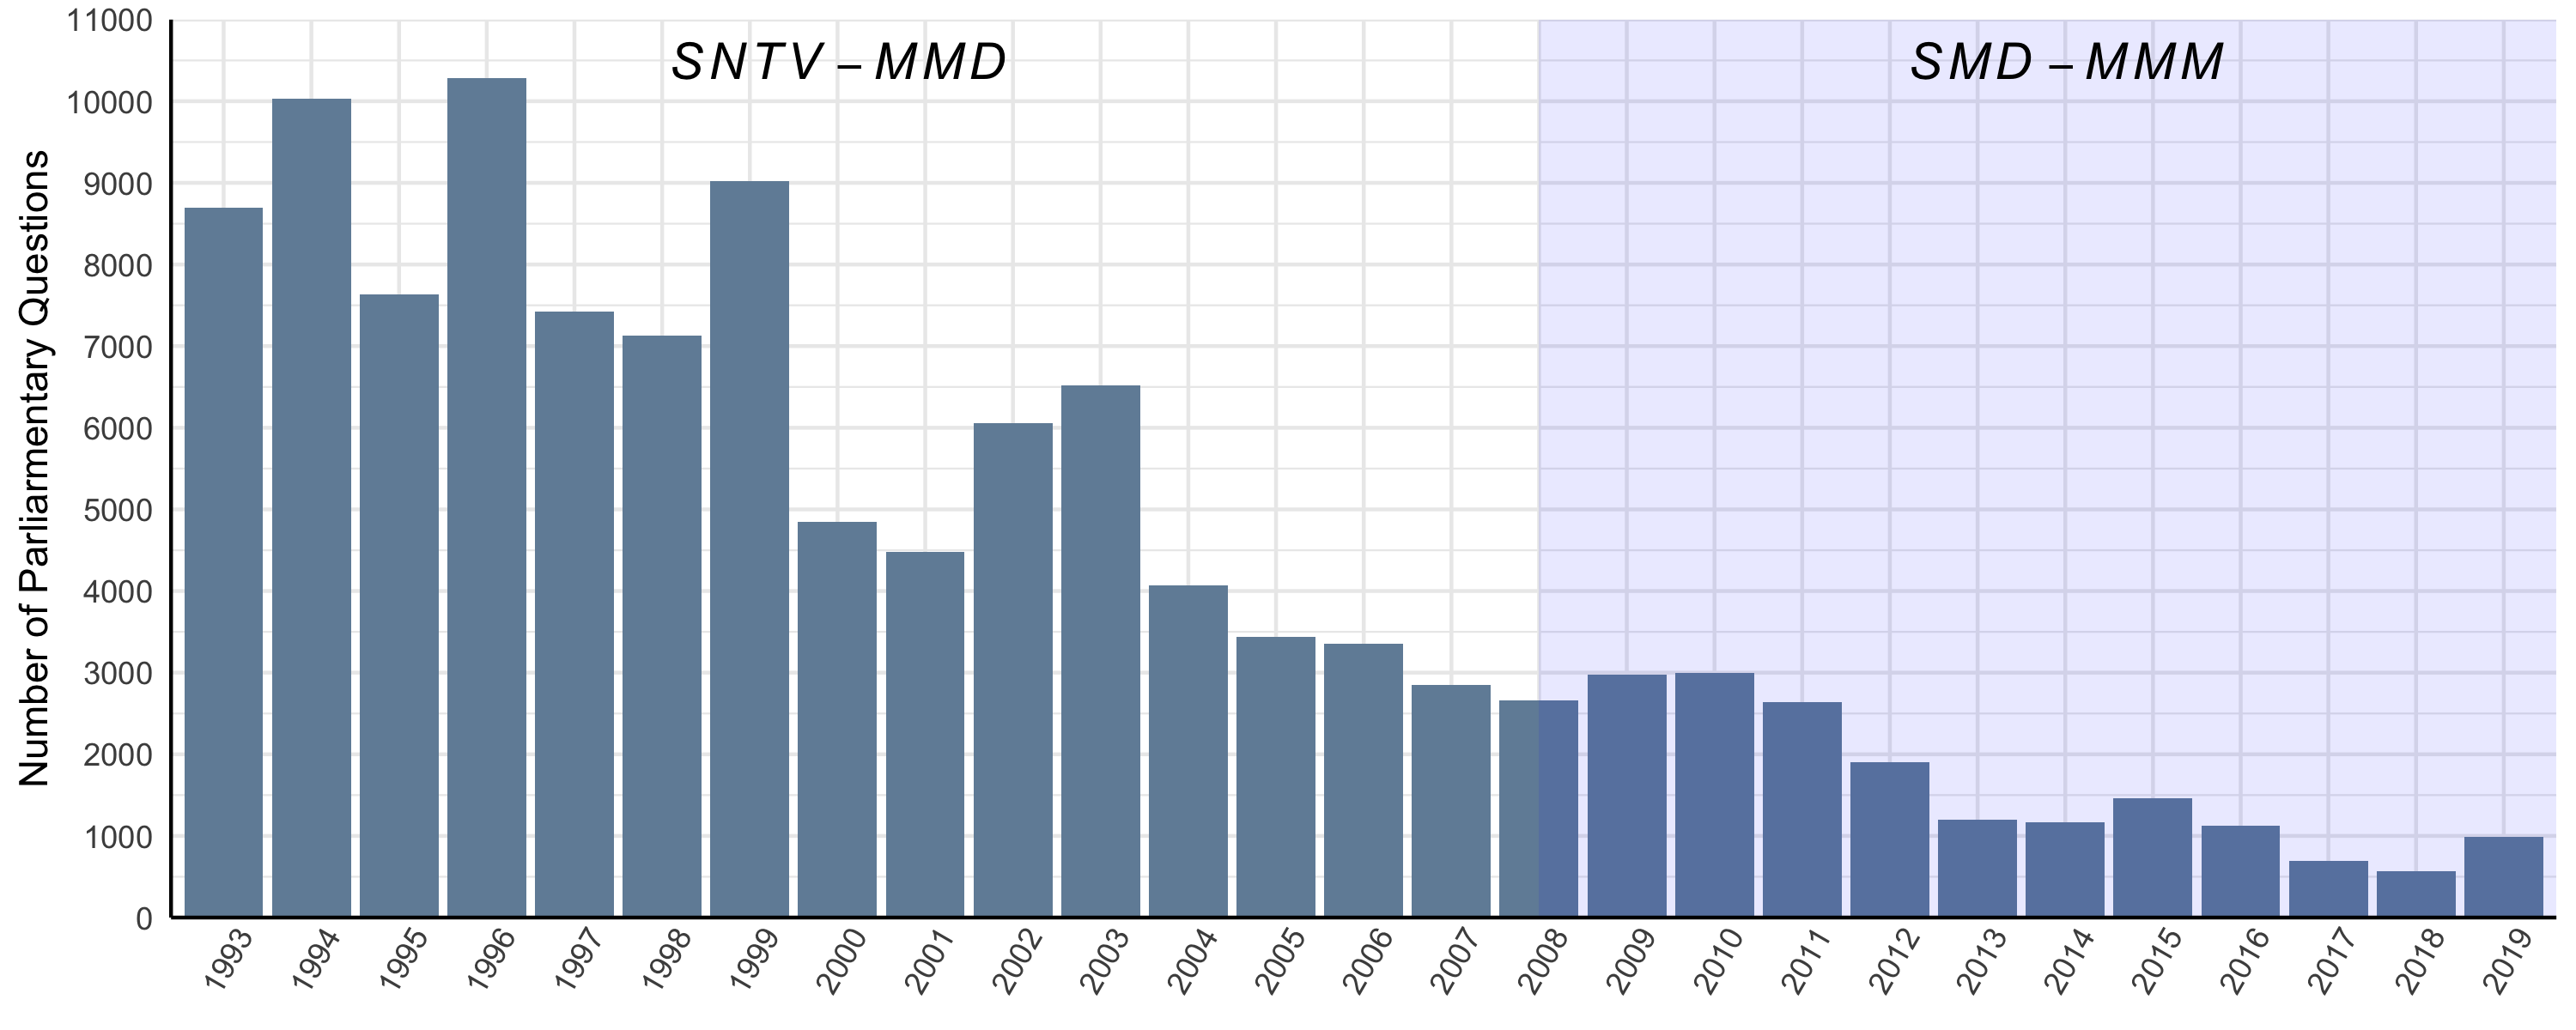
\includegraphics[width = 14.5cm, height=7.5cm]{03-Chapter-Three/image/p1.png}
    \caption{The Number of Parliamentary Questions from 1993 to 2019}
    \label{fig:pq}
    \begin{tablenotes}
    \end{tablenotes}
\end{figure}


To display the distribution of the questions across years, \autoref{fig:discriptionpq} demonstrates the total number of parliamentary questions documented from 1993 to 2019. During this period, the Taiwan legislature went through the movement of reducing legislative seats, which started in 2000, and the reform occurred in 2008. In the pre-2000 period, the number of questions asked remained roughly stable with multiple fluctuations. Nevertheless, there was a noticeable drop in the number of questions since 2000, right after the start of the movement. This trend persisted, and the total number of questions plummeted. 

The \autoref{fig:top20} shows the top 20 categories of topics that were frequently asked during the period. Topic categories related to social administration and police administration were the top two topics that appeared in the discussions in the legislature. Coming next are categories about environment and finance. 

\begin{figure}[hb!]
    \centering
    \begin{subfigure}[t]{0.48\textwidth}
    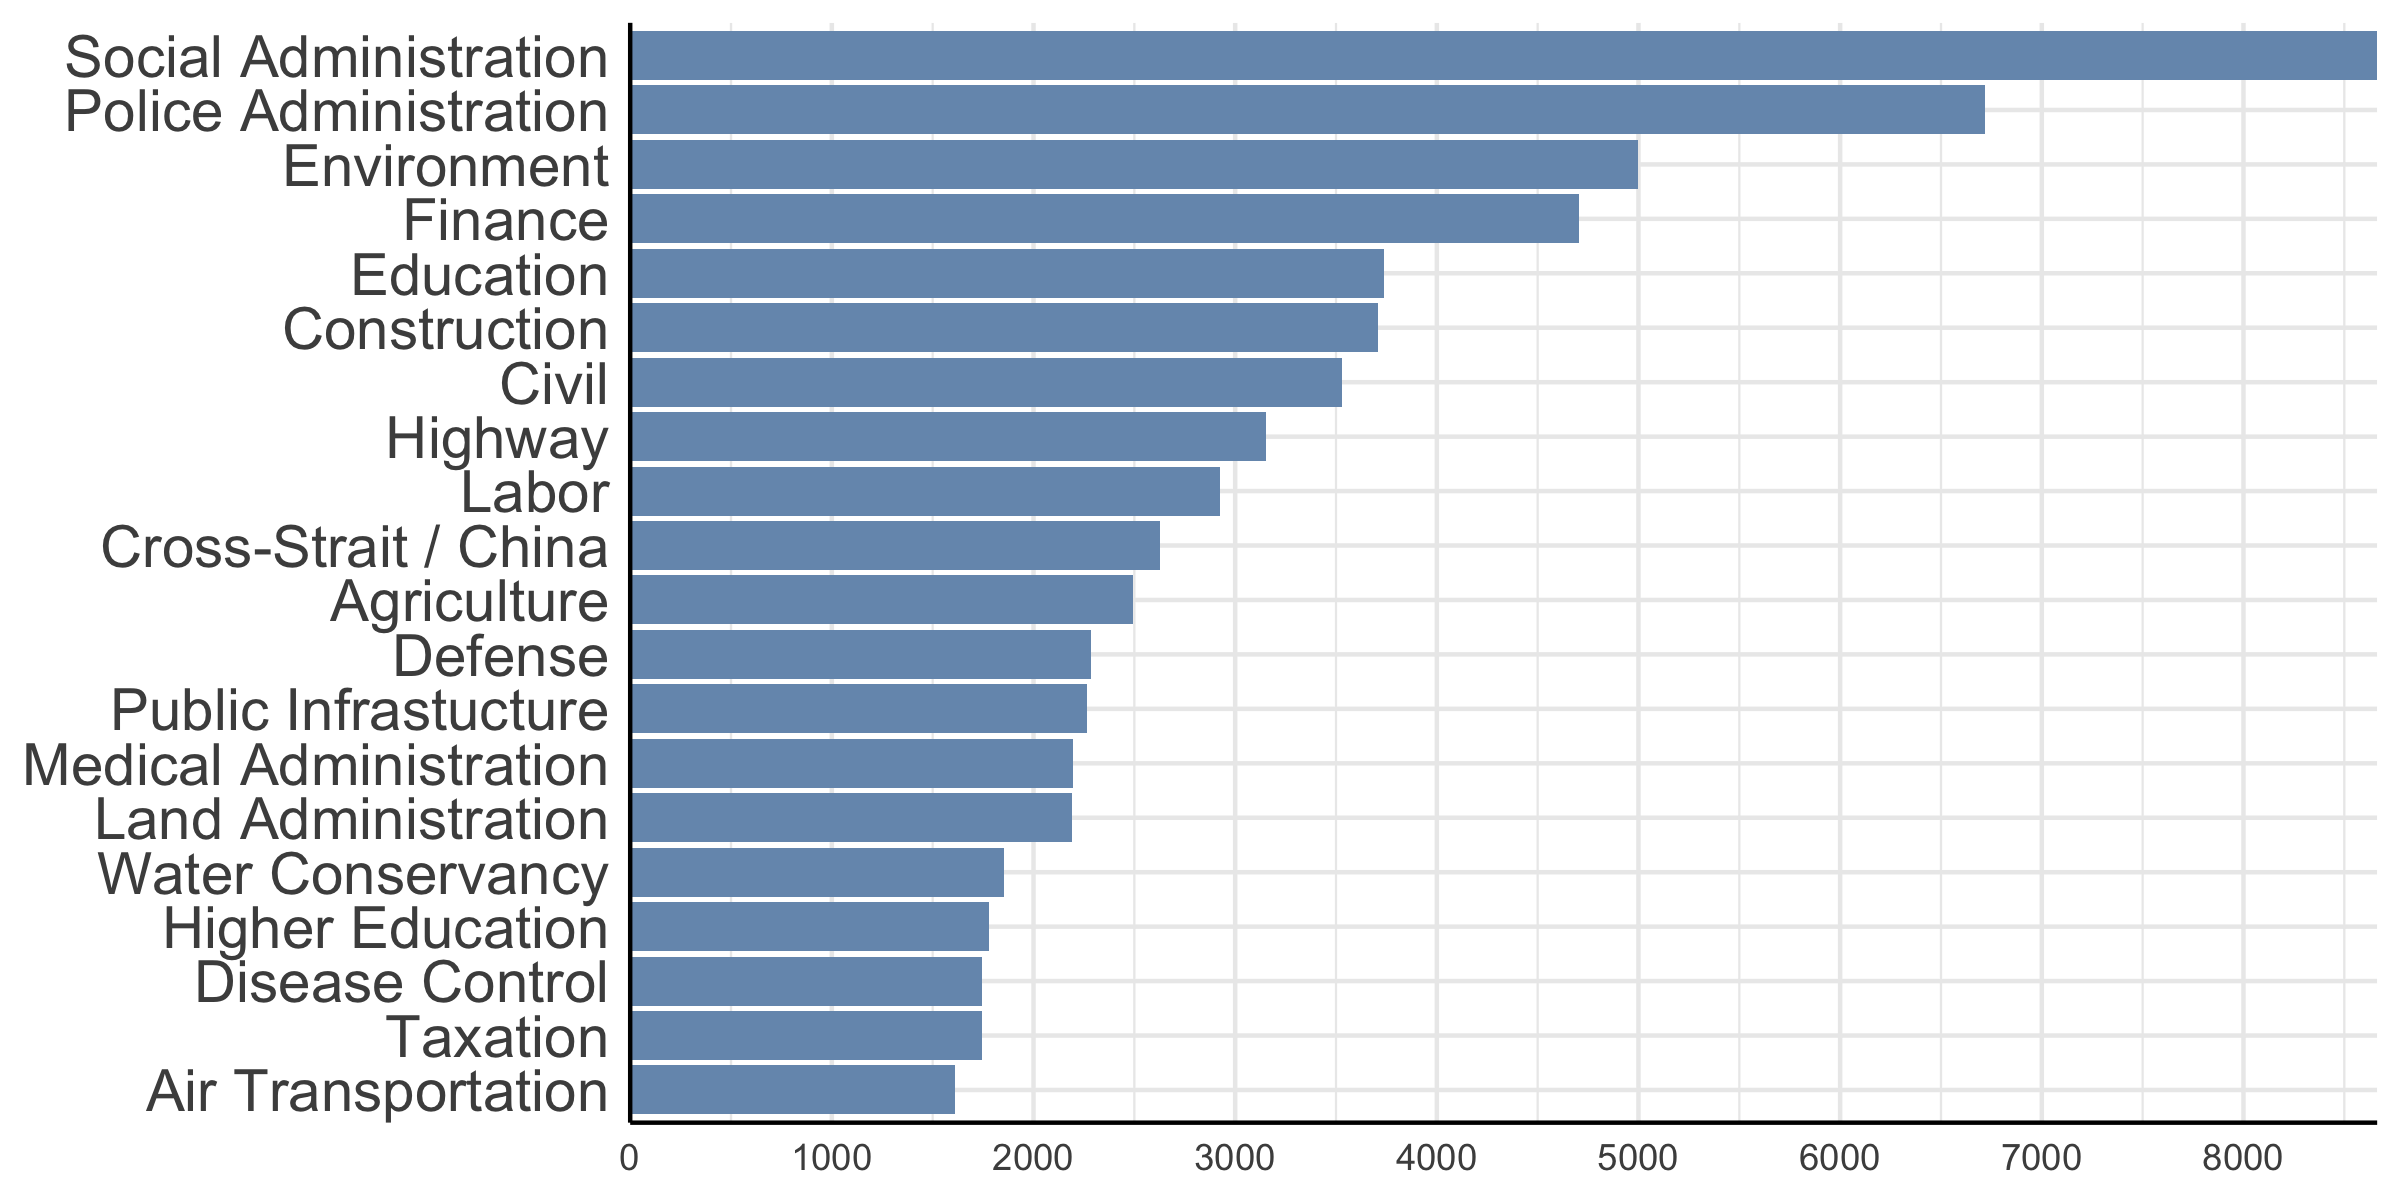
\includegraphics[width=7cm, height=5.6cm]{03-Chapter-Three/image/top20.png}
    % \caption{The Number of Parliamentary Questions from 1993 to 2019} 
    \caption{Tops 20 Most Frequent Categories} 
    \label{fig:top20}
    \end{subfigure}
    \centering
    \begin{subfigure}[t]{0.48\textwidth}
    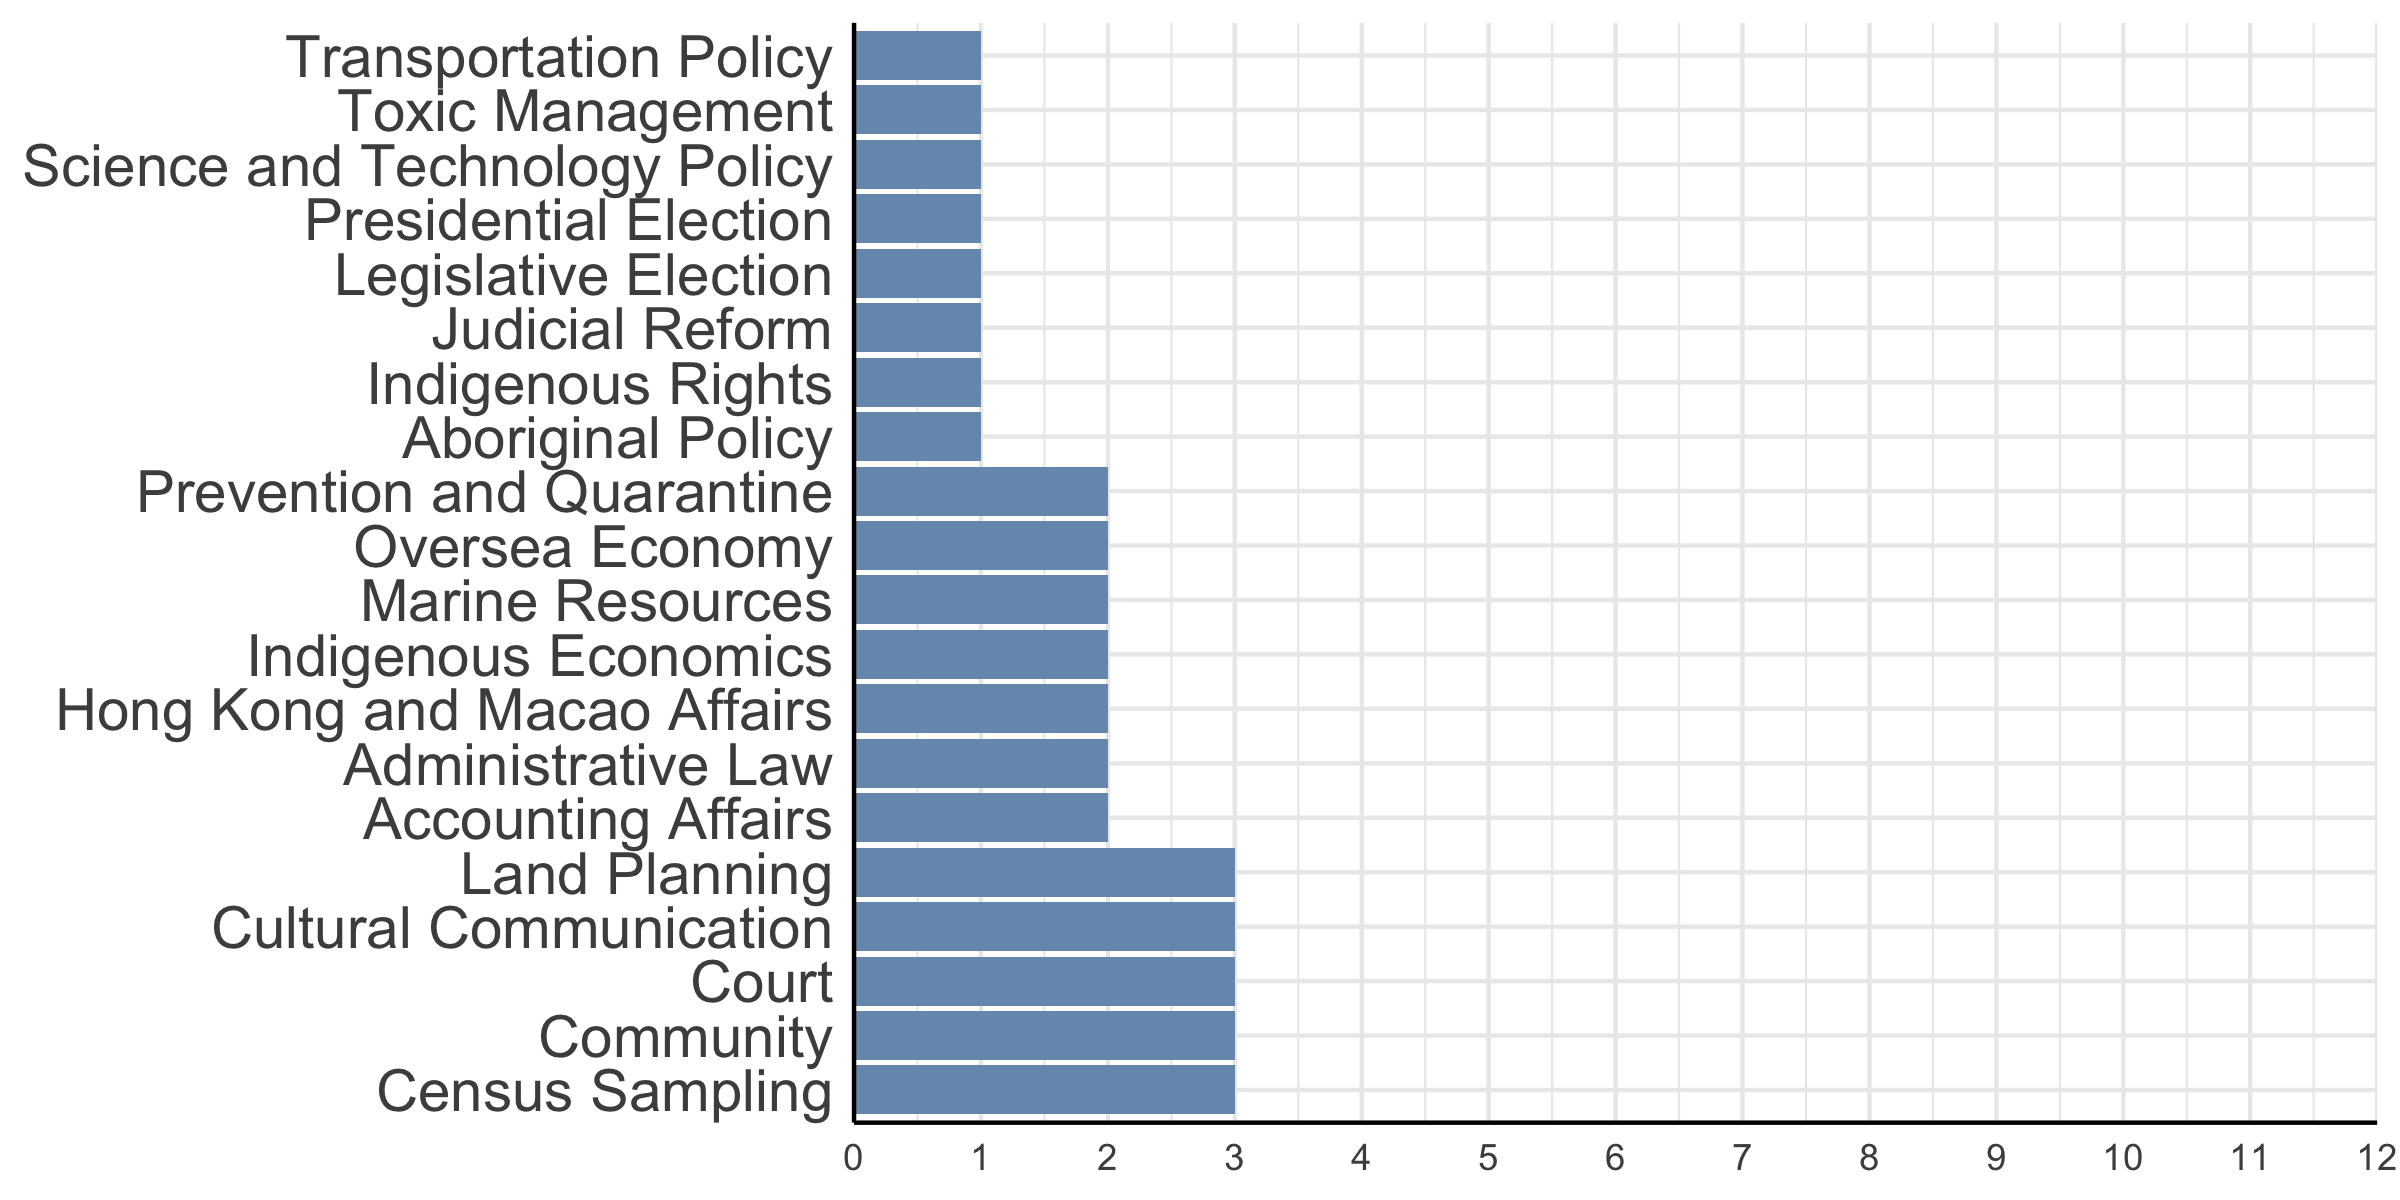
\includegraphics[width=7cm, height=5.6cm]{03-Chapter-Three/image/tail20.png}
    \caption{Top 20 Less Frequent Categories}
    \label{fig:tail20}    
    \end{subfigure}
    \caption{The Distribution of Parliamentary Questions Categories Asked by Legislators}
    \label{fig:discriptionpq}    
\end{figure}


\section*{\centering Pork Barrelling Machine Classifier}

This chapter takes advantage of using the Pork-barrel Legislation Dataset assembled by Prof. Dr Ching Jyuhn Luor \citep{Luor2008, Luor2009, Luor2012} to train the deep learning model proposed by this chapter. The collection of the dataset consists of 7243 pieces of legislation which were manually annotated as \textit{Pork (with label 1)} or \textit{Non-Pork (with label 0)} from 2004 to 2008. In addition, this data set was cross-coded by three social science researchers to assess its validity, which achieves 98\% in terms of consistency and precision among coders \citep{Luor2008,Luor2009}. 

\begin{figure}[!ht]
    \centering
    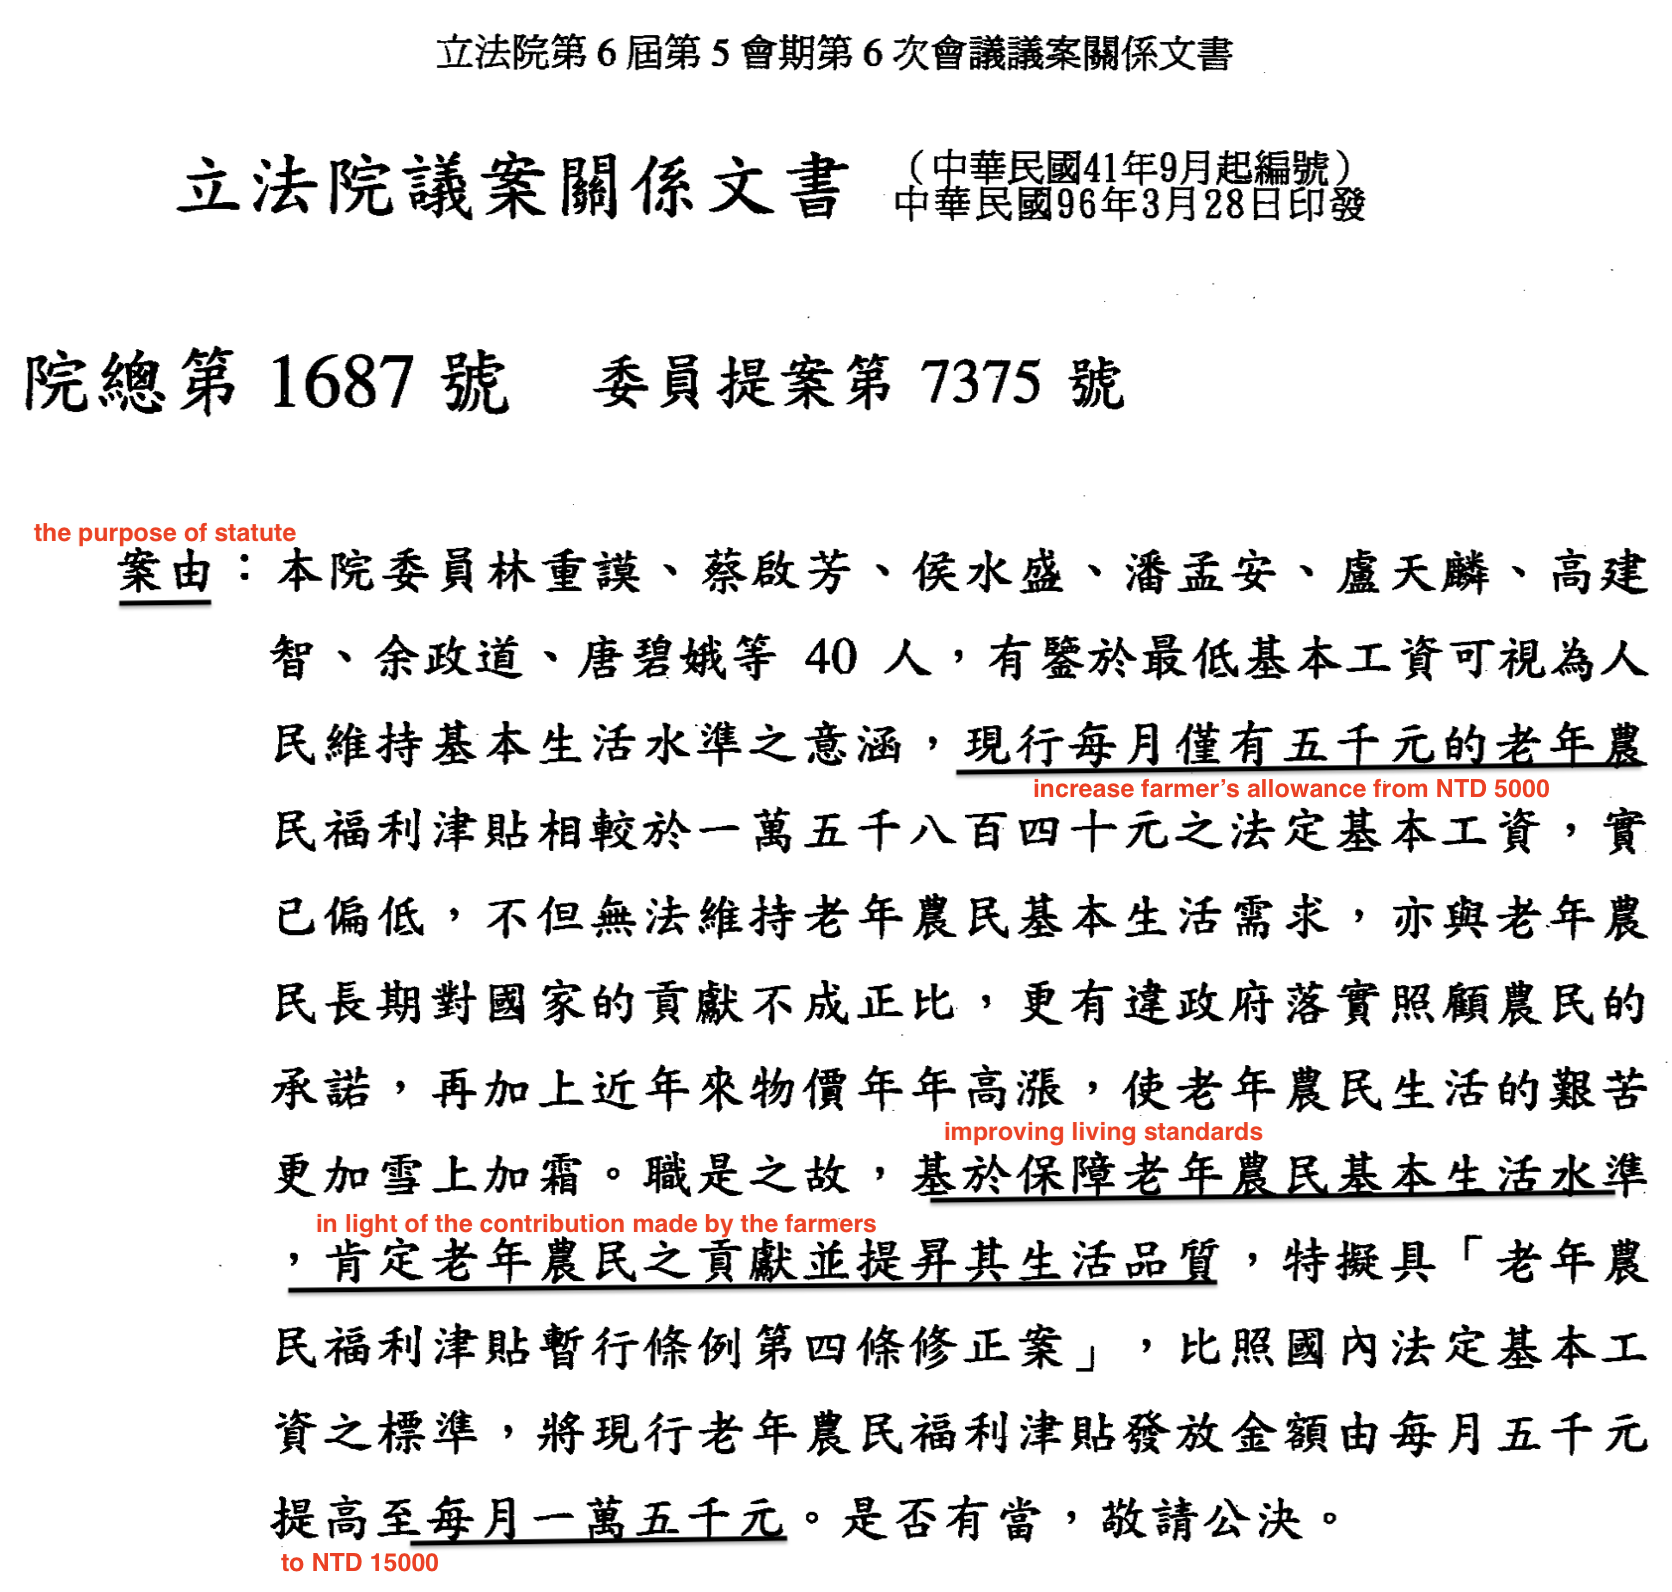
\includegraphics[width = 14.5cm]{03-Chapter-Three/image/billeg.png}
    \caption{Pork Barrel Legislation Regarding Improving the Quality of Retired Farmers' Life}
    \label{fig:farmers}
    \begin{tablenotes}
    \end{tablenotes}
\end{figure}


The gold standard for identifying pork barrel legislation is based on the target beneficiaries of the policy (distributed vs. concentrated) and the attributes of policy cost (distributed vs. concentrated), as illustrated in \autoref{fig:type}  \citep{Wilson2001}. In particular, typical pork-barrel policies (or legislation) mainly incur distributed costs while generating parochial benefits for specific regions or designated population groups. For instance, the decision to execute an areotropolis project, which involves constructing an airport within a particular area, e.g. Taoyuan City, incurs collective costs for all Taiwanese taxpayers, while the benefit of such a particularistic project is narrowly concentrated within a parochial group of Taoyuan residents (in terms of employment opportunities, economic development, and convenience of the airport) as well as local politicians such as legislators themselves \citep{Luor2008, Luor2009, Luor2012}. 

Moreover, another example is the subsidy for the targeted populations. As illustrated in \autoref{fig:farmers}, the purpose of the legislation was to raise the farmers' monthly allowance from NTD 5000 to NTD 15000. In general, the majority of retired farmers are concentrated in agricultural municipalities. Thus, \citet{Luor2008, Luor2009} operationalises those concepts commonly found in Taiwan's political context and further categorises the legislation into pork and non-pork.

\begin{figure}[ht]
    \centering
    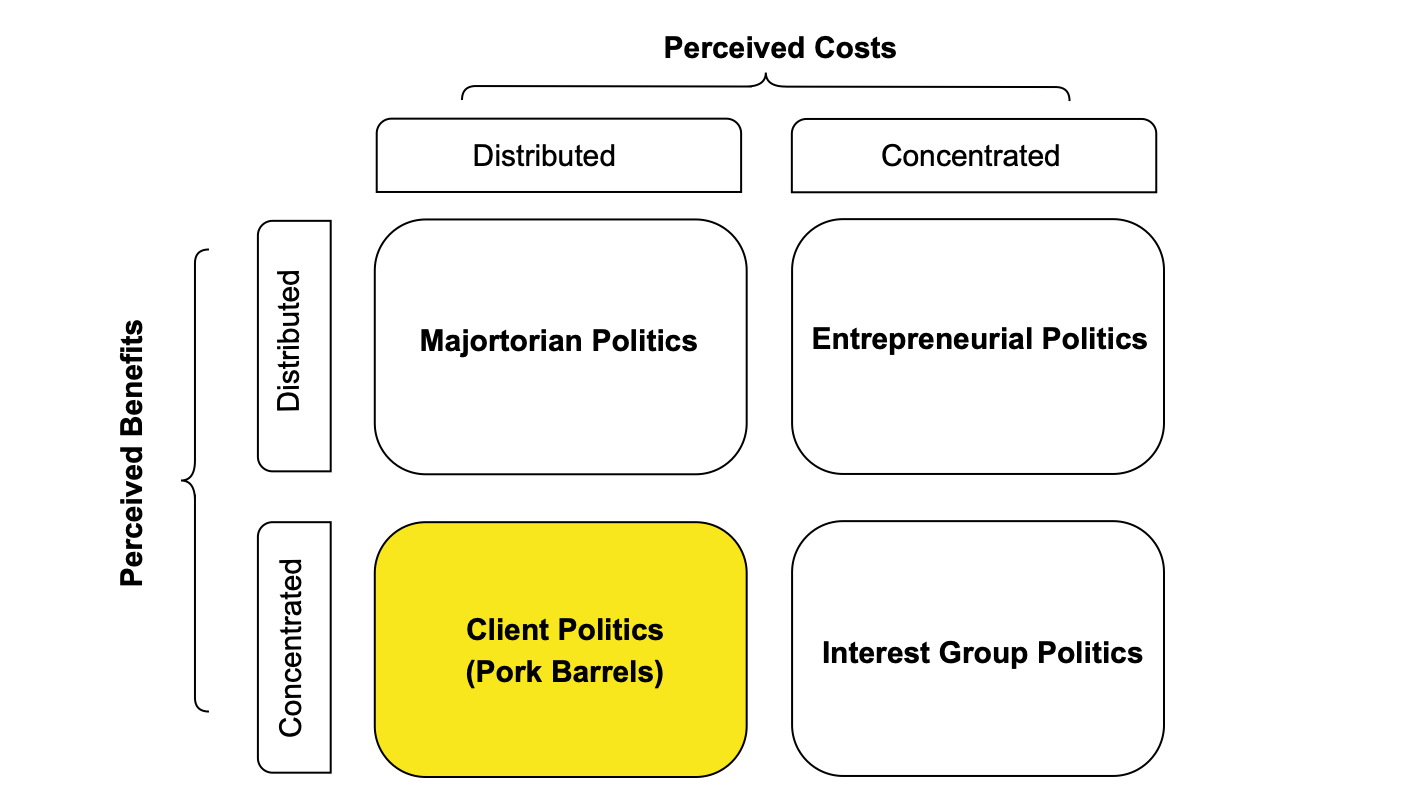
\includegraphics[width = 17cm, height=10cm]{03-Chapter-Three/image/porktype.png}
    \caption{Classifying and Explaining the Politics of Different Policy Issues, Source: \citet{Wilson2001}}
    \label{fig:type}
\end{figure}


\subsection*{Using BERT Model as Embedding Layers}

With increasingly available amounts of political data, the application of the classification task using deep learning methods has received great attention in political science \citep{Chatsiou2020}. In natural language processing, text classification assigns a set of predefined categories to open-ended documents. The approach used in this chapter is to combine one of the famous Transformer architectures, BERT developed by Google, with convolutional neural networks. 

CNN is one of powerful neural network architectures commonly applied in natural language processing \citep{Zhang2015, Zhang2020, Kim2014, Kim2016}. The architecture can be constructed by a series of convolutions and pooling layers, filtering input vectors and creating a feature map that summarises the input texts. Then, the feature map can be stacked one over another to form a matrix by single-dimensional convolutional filters to extract high-level features. In the context of text classification task, convolution layer essentially learns the condensed features as learning image data. 

\begin{figure}[ht]
    \centering
    \begin{subfigure}[t]{0.45\textwidth}
    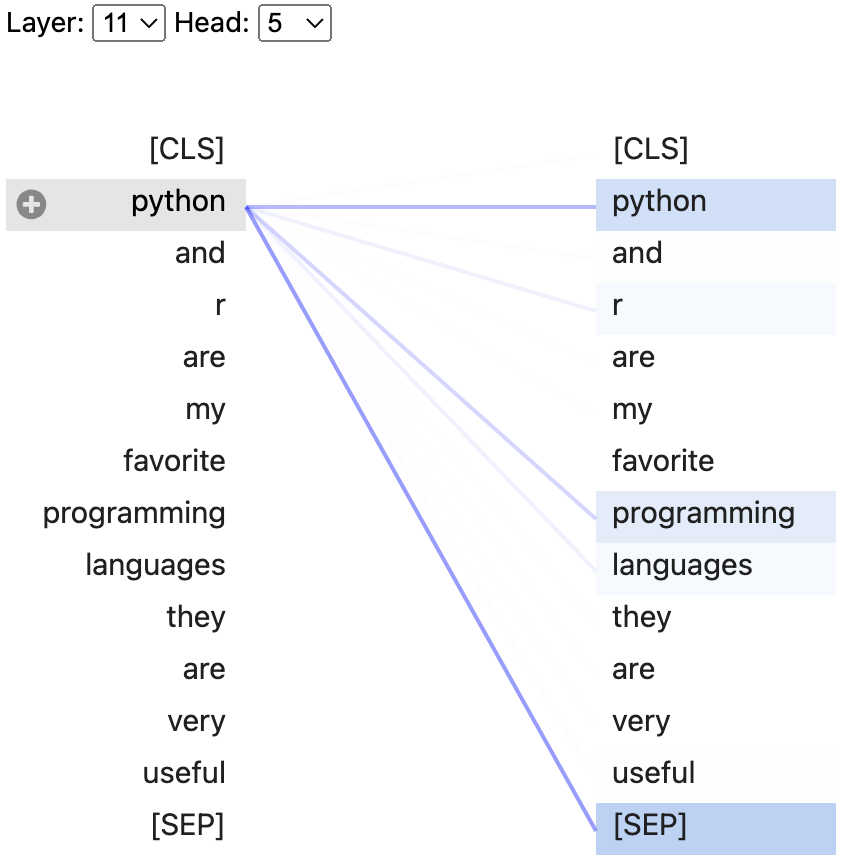
\includegraphics[width=7cm, height=6cm]{03-Chapter-Three/image/vis2.png}
    \caption{Sentence 1: Python refers programming language}
    \label{fig:python1}
    \end{subfigure}
    \centering
    \begin{subfigure}[t]{0.45\textwidth}
    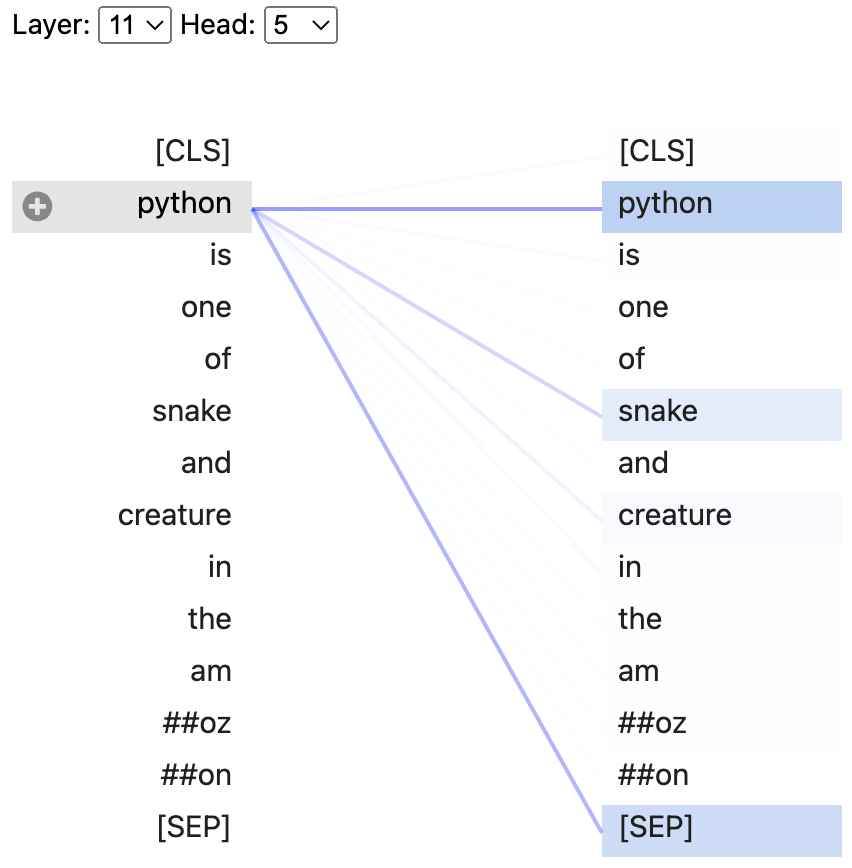
\includegraphics[width=7cm, height=6cm]{03-Chapter-Three/image/vis3.png}
    \caption{Sentence 2: Python refers snake}
    \label{fig:python2}    
    \end{subfigure}
    \caption{An Example of Self-attention Mechanism in BERT  Transformer Using 
    Pretrained model on English language (\href{https://huggingface.co/bert-base-uncased}{bert-base-uncased})
    % \footnote{Visualization using BertViz library\citep[see,][]{vig-2019-multiscale}}
    }
    \label{fig:visbert}    
\end{figure}

In practice, the convolutional layers (or recurrent neural net) are recently introduced as encoders or decoders to deal with semantics problems in modern application of natural language processing. Generally, we can transform input texts with embedding models such as Word2Vec, GloVe or one-hot vector. However, the major challenge of these approaches lies in the fundamental assumption that each input word has fixed representation in different contexts, introducing a potentially severe problem of misrepresentations by referring to inaccurate meaning across sentences. For example, the embedding word ``python'' as shown in \autoref{fig:visbert} can have different meanings depending on the language context in which it appears. Regardless of polysemous mean in different sentences, the word ``python'' only renders the same vector. This is because traditional embedding models are context-free, which gives static embedding vectors for the word ``python''. 

Contrary to earlier approaches, BERT is one of the most powerful Transformer architectures that can detect input tokens in bidirectional semantic context with its prominent feature called self-attention \citep{Devlin2019, Vaswani2017}.\footnote{BERT is the first contextual-based model based on the transformer architecture released by Google.  Transformers models also include ALBERT, RoBERTa, DistilBERT, GPT2 and others.} Theoretically, BERT consists of 12 encoder layers, stacked over one another as shown in \autoref{fig:bert}, respectively. For example, giving the single word ``python'' in two different contexts in \autoref{fig:visbert},  ``python'' in \autoref{fig:python1} refers to one of the programming languages because contextual embedding is highly associated with ``programming'', ``languages'', and ``r (statistical computing language)''. On the other hand, ``python'' in \autoref{fig:python2} refers to an animal in the sentence context as its representation embedding is correlated with snake and creature.

As discussed above, self-attention is a mechanism that allows neural networks to assign a different amount of attention weight to each element to compute representation embedding in a sequence. This is powerful for performing NLP tasks when dealing with unseen words or tokens not included in the static embedding model like Word2Vec.   

\begin{figure}[htbp]
    \centering
    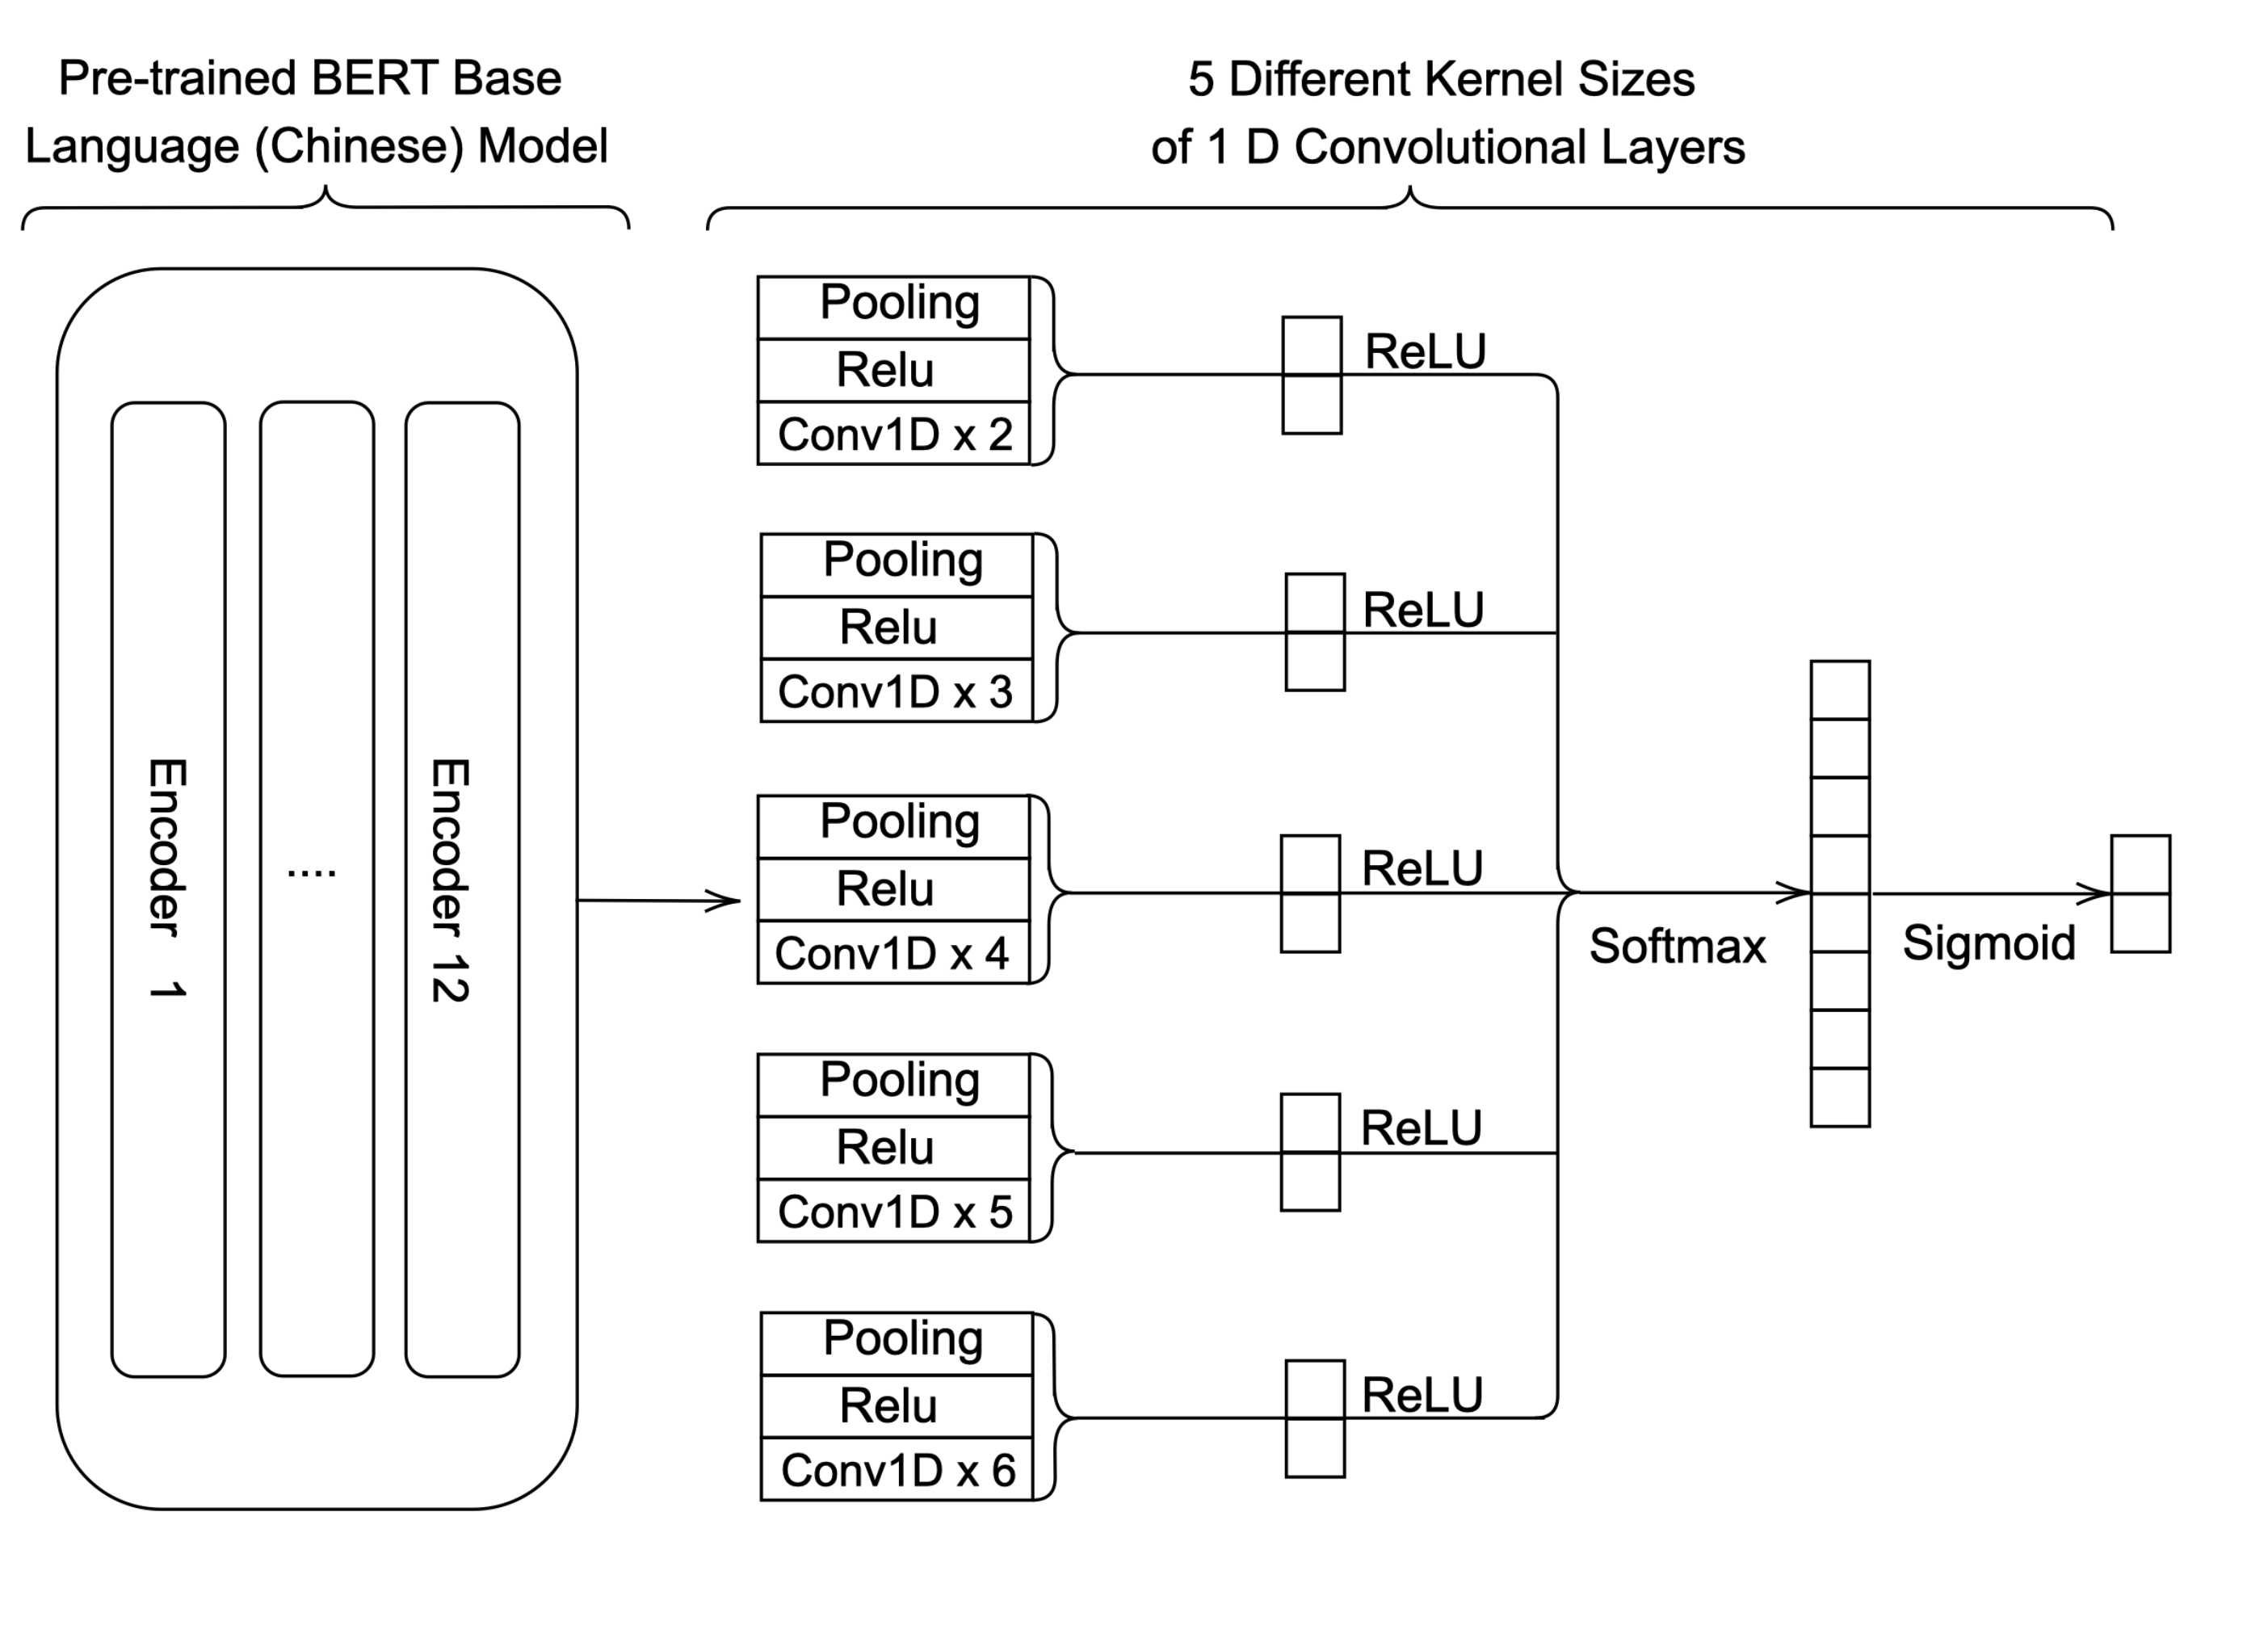
\includegraphics[width = 14.5cm, height=9.1cm]{03-Chapter-Three/image/framework.png}
    \caption{The Designed Architecture for Pork Barrel Classification Task}
    \label{fig:bert}
    \begin{tablenotes}
    \end{tablenotes}
\end{figure}

\subsection*{Combining Convolutional Neuralnet with BERT Embedding Layer}
Combining CNN with BERT for classification tasks is getting popular in natural language processing in recent years \citep{Safaya2020, Lu2019, Lopez2017}. For example, \citet{Safaya2020} use convolutional layers followed by BERT embedding to create a machine learning model that deals with offensive speech identification, while \citet{Lu2019} deploying the similar approach to patent document classification. Those performance of combination approach is drastically improved from the character-based CNN and the generic BERT model, respectively. The innovative design for machine learning architecture in the literature that motivates the model used is the following. I create the architecture for detecting pork-barrel features in parliamentary questions, as shown in \autoref{fig:bert}. All the encoders use 12 attention heads and 12 layers. Theoretically, each token can be represented as 768 hidden units \citep[][]{Wolf2020}.\footnote{The traditional Chinese BERT model used in the chapter is \textit{bert-base-Chinese} which is maintained by CKIP (Chinese Knowledge and Information Processing) at the Institute of Information Science and the Institute of Linguistics, Taiwan Academia Sinica.} 

First, I transform each word in the sentence with its word vector using the Chinese BERT pre-trained model.\footnote{This model can be downloaded from \href{ https://ckip-transformers.readthedocs.io/en/stable/}{ https://ckip-transformers.readthedocs.io/en/stable/} and \textit{HuggingFace} at \href{https://huggingface.co/bert-base-chinese}{https://huggingface.co/bert-base-chinese}.}  In the BERT layer, I can feed input sentences (pork legislation text) in the encoder layer, where the encoder learns the representation. Afterwards, the decoder generates new output based on the patterns understood by the following encoder. In order to fit embedding vector into CNN layers, I create five kernels of different lengths, aiming to capture different patterns of the n-gram in the original sentence. After the output is passed through ReLU activation, Global Max Pooling is introduced to flatten high-dimensions feature maps into two-dimensional vectors. At the last set of layers, I use the Sigmoid function commonly adapted for binary class with dense layers to get the final outcome, which is the probability of being classified as pork-barrel project.\footnote{Regarding the metrics of model performances, see \autoref{tab:performance} in Supplementary Appendix \ref{tag:performance}. }



\begin{table}[h]
\caption{Sampled Parliamentary Questions Being Most Likely to Mention Particularistic Goods}
\centering
\scalebox{0.68}{
    \begin{tabular}[t]{l*{4}{c}} 
    \toprule 
    Legislators               & 
    Probability of Being Pork &   
    Topics                    &
    Keywords                  &
    Questions \\ [0.8ex]
    \hline
    林正峰 & 0.995515823364258 & Health Insurance     & Health Insurance Deductions & 特别扣除额教育支出...\\
    彭添富 & 0.992780447006226 & Aboriginal Affair    & Housing Subsidies & 
    而非采用扣除免税额...\\
    李復興 & 0.992780089378357 & Old-age Benefits     & Elderly Allowance & 
    原住民家庭租屋補助...\\
    盧秀燕 & 0.992639720439911 & Veterans Welfare     & Grants for Retired Veterans & 
    補助金發放金額過低...\\   
    李顯榮 & 0.990033149719238 & Farmer Welfare       & Subsidies; Allowance  & 
    政府前後援賽金額高...\\   
    丁守中 & 0.988385319709778 & The Handicapped      & Living Allowance  & 
    身心障礙者生活津貼...\\   
    馮定國 & 0.985531985759735 & Elderly Welfare      & Unemployment Fund &
    高齡失業問題嚴重日...\\   
    彭添富 & 0.983698368072510 & Agriculture          & Crops Subsidies &
    農作物損失補償問題...\\   
    曾華德 & 0.979519009590149 & Military Affair      & Increased Pay  &
    救国军补发薪饷问题...\\   
    林鴻池 & 0.978044390678406 & Education            & University Subsidy &
    針對諸多已獲得五年...\\   
    
        \bottomrule
        \end{tabular} }
    \label{table:pork}
\end{table}

To validate the classification quality, I sampled 20 pork and non-pork questions respectively in \autoref{table:pork} and \autoref{table:nonpork}, automatically classified by the architecture in \autoref{fig:bert}. I merge these questions with corresponding keywords and categories (translated to English) scraped from the website of Taiwan Legislative Yuan. As shown in \autoref{table:pork}, most pork-barrel questions are associated with central government spending for targeted groups and localised infrastructure projects mainly allocated to specific regions. Some legislators raise the question of asking the central government to increase rent subsidies for the aboriginal population, while others target policies related to relief and support programmes such as crop subsidy and elderly allowances for specific groups in some municipalities located in western Taiwan. In addition to \autoref{table:nonpork} demonstrate many examples of non-particularistic questions. For instance, the questions of keywords and topics are very closely related to regulatory and national policies such as railway management, drug control and criminal investigation. 

% Table \ref{table:pork} displays the most possible of being pork-barrel quantities, whereas Table \ref{table:nonpork} exemplifies the number of sample questions that are more likely to label non-pork-barrel features. 


\begin{table}[ht]
\caption{Sampled Parliamentary Questions Being Less Likely to Mention Particularistic Goods }
\centering
\scalebox{0.68}{
    \begin{tabular}[t]{l*{4}{c}} 
    \toprule
    Legislators               &
    Probability of Being Pork &   
    Topics                    &
    Keywords                  &
    Questions               \\ [0.8ex]
\hline
    李復甸 & 0.000021549063604 & Litigation Procedure & Criminal Investigation &
    鑑於刑事偵察實務上...\\
    林建榮 & 0.000020212990421 & Financial Management & Revolving Interest Rate &
    明定信用卡、現金卡...\\
    林正峰 & 0.000019731034627 & Energy Policy        & Energy Saving  & 
    要求各級機關和學校...\\
    林正峰 & 0.000019187420548 & Tobacco Restriction  & Departmental Hospital &
    毒品氾濫,吸毒人數...\\   
    王幸男 & 0.000017634354663 & Public Safety        & Road Quality & 
    針對道路人孔蓋或管...\\   
    管碧玲 & 0.000013002485503 & Railway Management   & Taiwan Railway &
    台灣鐵路管理局發生...\\   
    郭榮宗 & 0.000004869816621 & District Court       & Drug Abuse & 
    知名提神飲料遭下毒...\\   
    陳朝龍 & 0.000011277100384 & Infectious Disease   & Avian Influenza  &
    英國政府宣稱台灣出...\\   
    林進興 & 0.000007685628589 & Banking Management   & Credit Card  &
    行政院金融監督管理...\\   
    潘孟安 & 0.000002590457370 & Election             & Legislative Elections &
    單一選區兩票制即將...\\   
        \bottomrule
        \end{tabular} }
\label{table:nonpork}
\end{table}


\section*{\centering Heterogeneous Effects on Different Sizes of Parties}

I next examine the distribution of pork-barrel questions aggregated by party level from 1993 to 2019. \autoref{fig:sumpork} displays the distribution of the total number of pork-barrel questions that were requested by legislators from two major parties and the small parties, respectively, as is classified by the deep learning architecture. The left subplot for the two majority parties, KMT (Chinese Nationalist Party) and DPP (Democratic Progress Party), roughly shares a similar pattern as in \autoref{fig:pq}, with a decreasing trend of the numbers overtime after the initiation of the movement that started around 2000. The right subplot \autoref{fig:sumporksmall} shows the multiple plummets and rises 
in the total number of questions raised by small parties such as NP (New Party 新黨), PFP (People First Party 親民黨), NPSU (Non-Partisan Solidarity Union, 無黨團結聯盟), TIP(Taiwan Independence Party 台灣獨立黨), TSU(Taiwan Solidarity Union 台灣團結聯盟) and newly established MKT (the Republican Party as known as Minkuotang).

\begin{figure}[ht]
    \centering
    \begin{subfigure}[t]{0.48\textwidth}
    \centering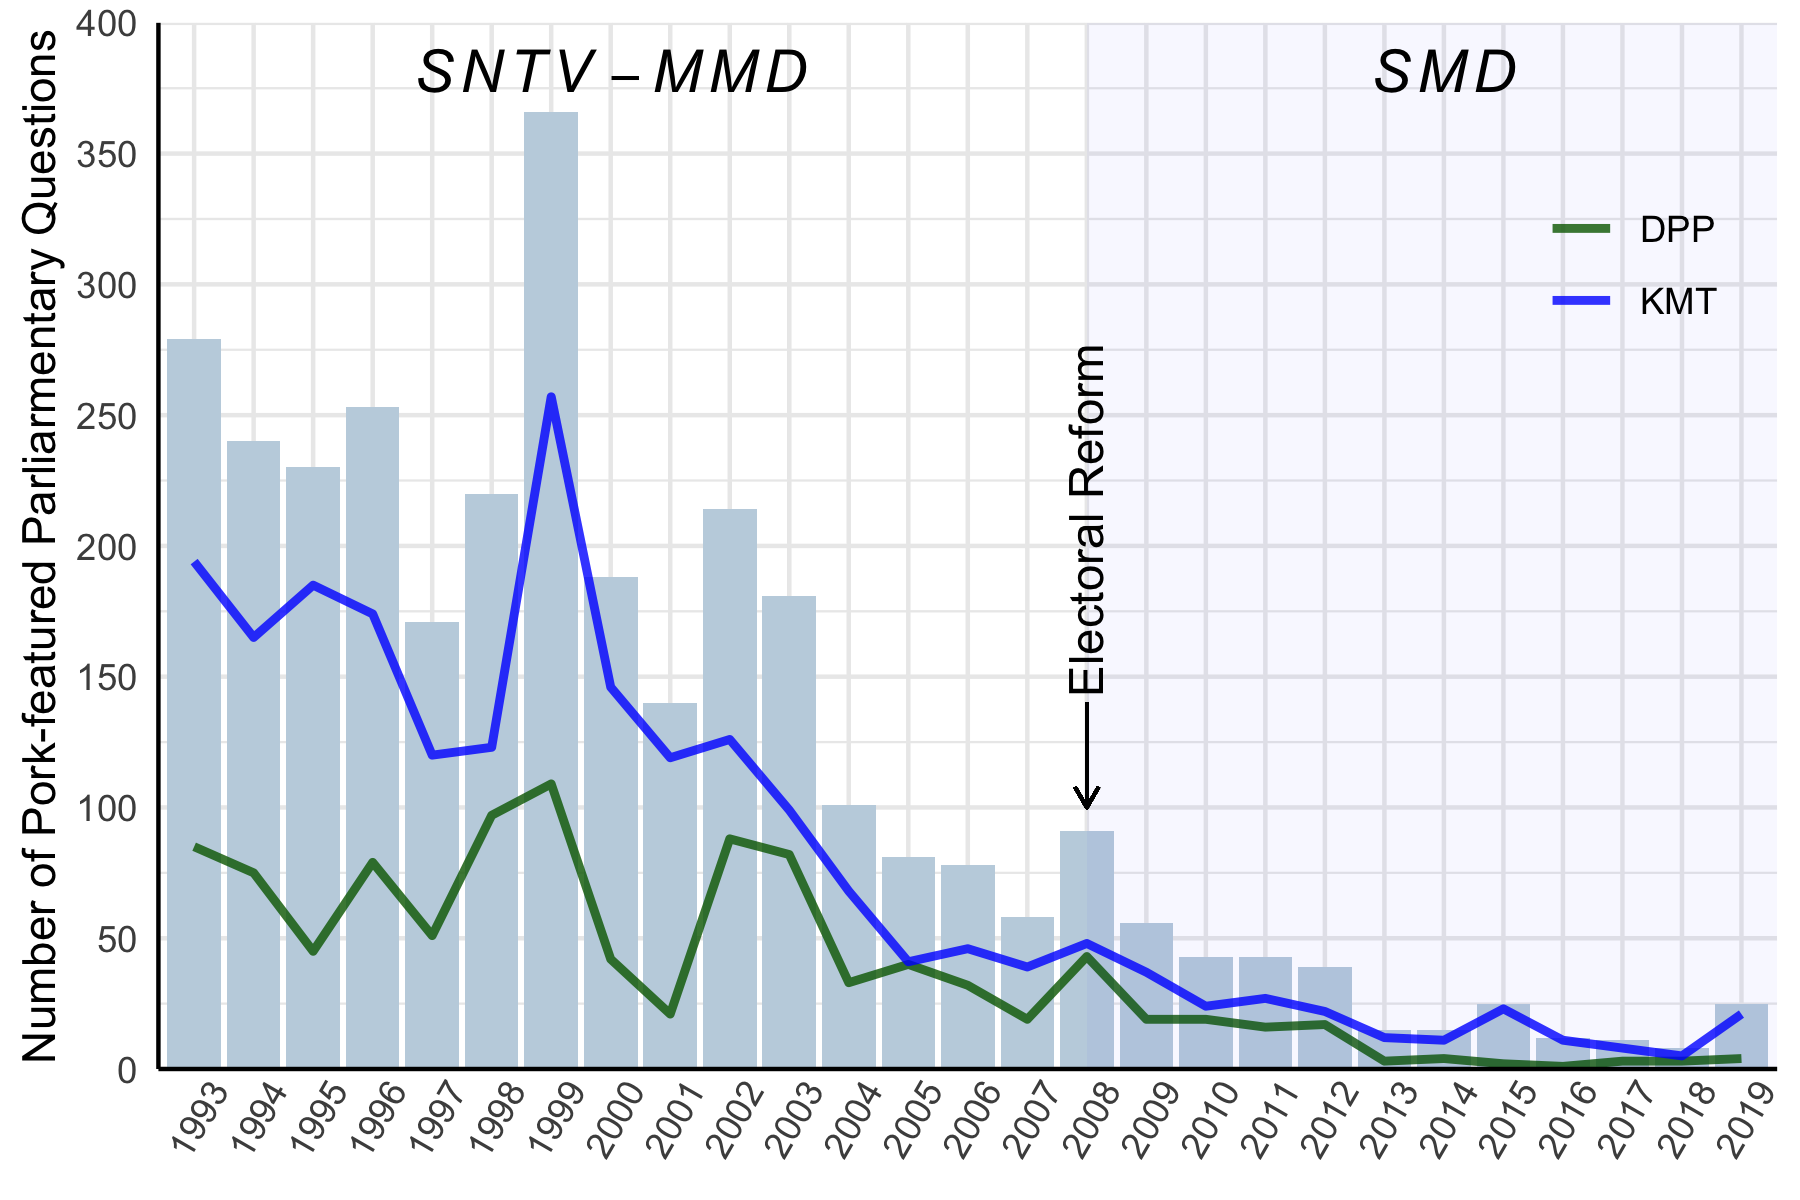
\includegraphics[width=7.2cm, height=6cm]{03-Chapter-Three/image/bigpq.png}
    \caption{Large Parties}
    \label{fig:sumporkbig}
    \end{subfigure}
    \begin{subfigure}[t]{0.48\textwidth}
    \centering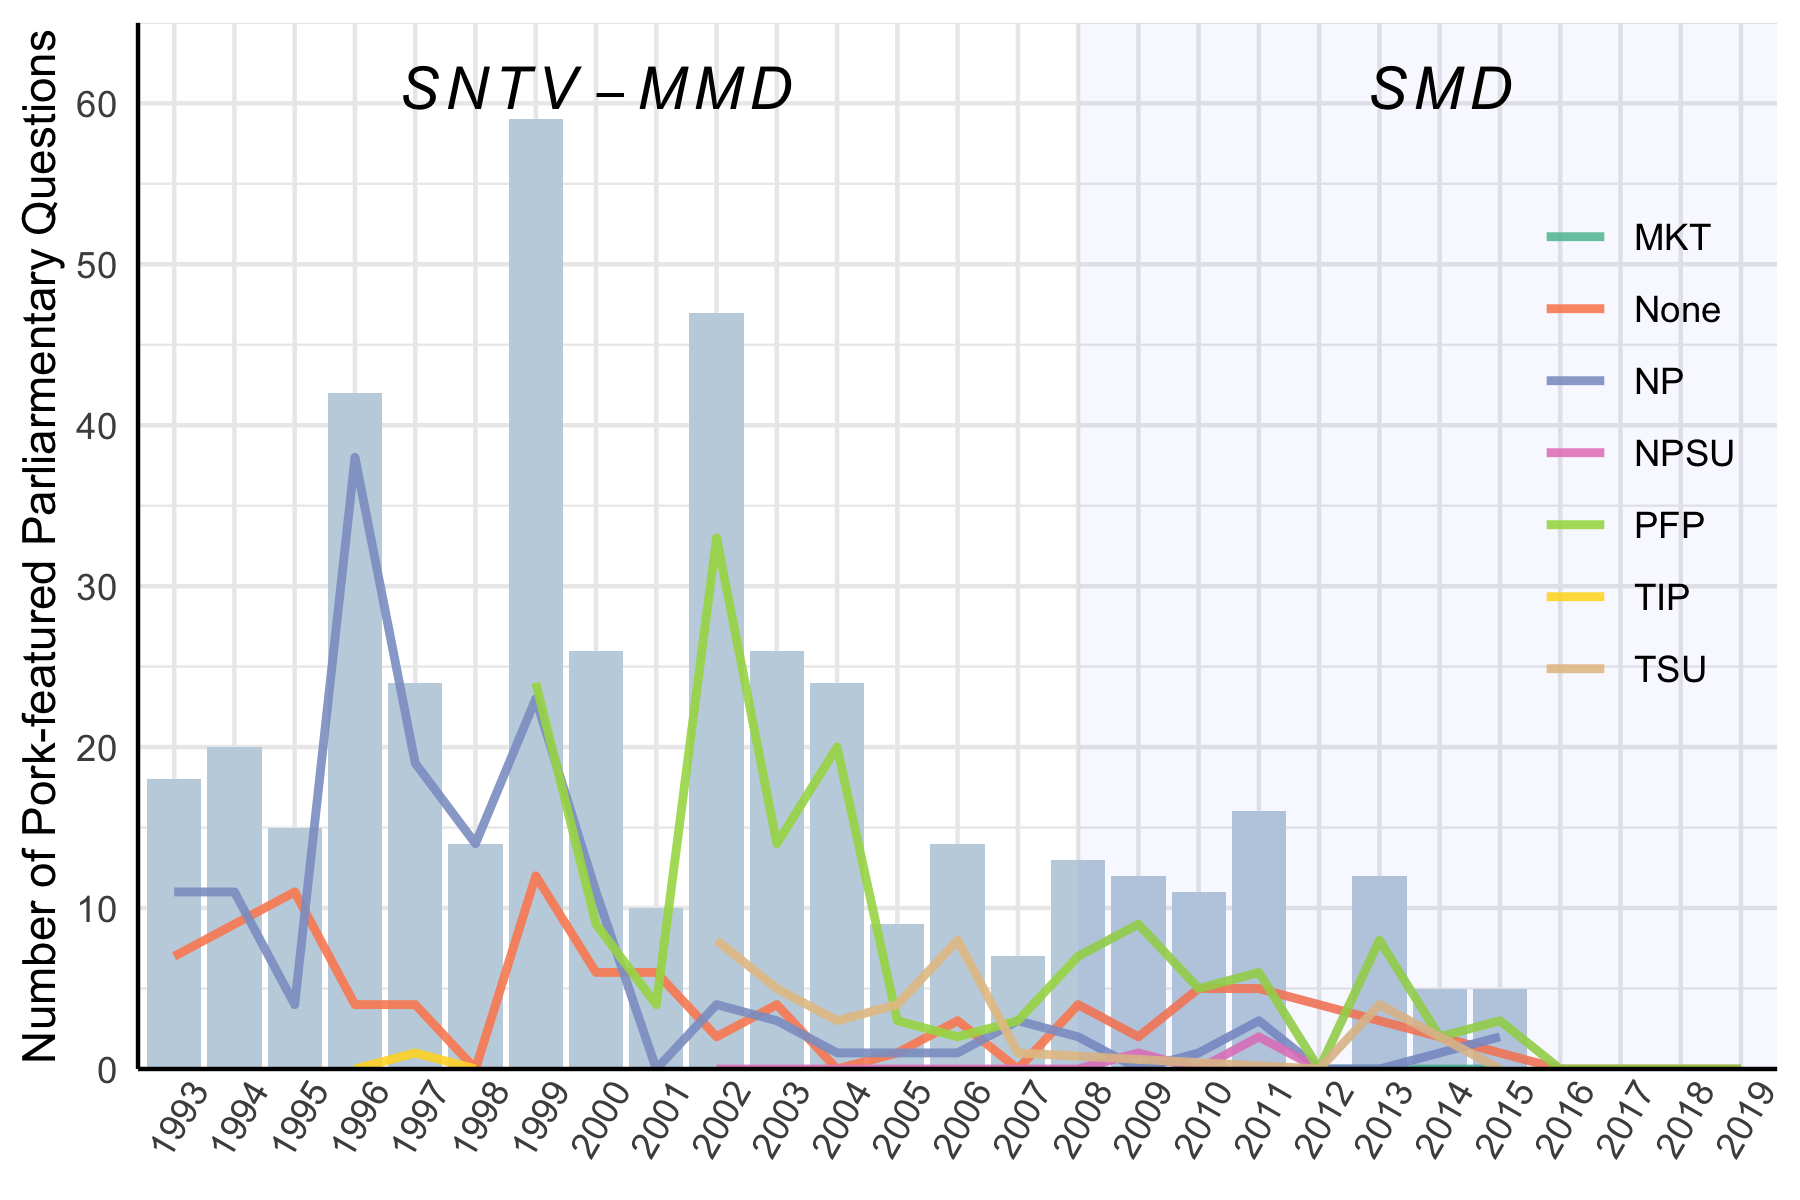
\includegraphics[width=7.2cm, height=6cm]{03-Chapter-Three/image/smallpq.png}
    \caption{Small Parties}
    \label{fig:sumporksmall}    
    \end{subfigure}
    \caption{The Number of Pork Barrel Question by Years}
    \label{fig:sumpork}    
\end{figure}


For \autoref{fig:sumpork}, the changes in the total numbers across times show that parliamentary questions are dwindling steadily, implying that legislators may alternatively use other tools to influence policy for their constituents, such as social media. For example, empirical evidence shows that district members mention more geographical terms on their Facebook and Twitter, whereas party-list members have less tendency to secure pork-barrel projects. In particular, the total number of seats was reduced from 225  to 113 after the reform. In the new system, only  73 seats are elected by district, explaining a fall-off in the number of pork-question since the reform occurred in 2008.

To exclude the effect of volatility in the number of seats across years, I illustrate the average number of pork-barrel questions per seat in the legislature. \autoref{fig:meanpork} plots the average number of questions per seat devoted to pork-barrel project for majority parties (\autoref{fig:meanporkbig}) and small parties (\autoref{fig:meanporksmall}), respectively. The actual impacts of the reform seem heterogeneous on small parties and large parties (KMT and DPP). In \autoref{fig:meanporkbig}, for large parties, the average number persistent declined from around 2001 to 2015, although there was a significant bounce back since 2017. Generally speaking, there are variations in the number of pork questions asked by small-party legislators, compared with legislators from KMT and DPP. From 2003 to 2012, the number of pork questions asked by each legislator from small parties was twice the size of large-party legislators. However, the reform differed from what I expected regarding small-party legislators: their average number increased from 2001 to 2009, yet this trend stopped in 2007. Afterwards, the trend became downward sloping, and the average number kept declining.

\begin{figure}[!ht]
    \centering
    \begin{subfigure}[t]{0.48\textwidth}
    \centering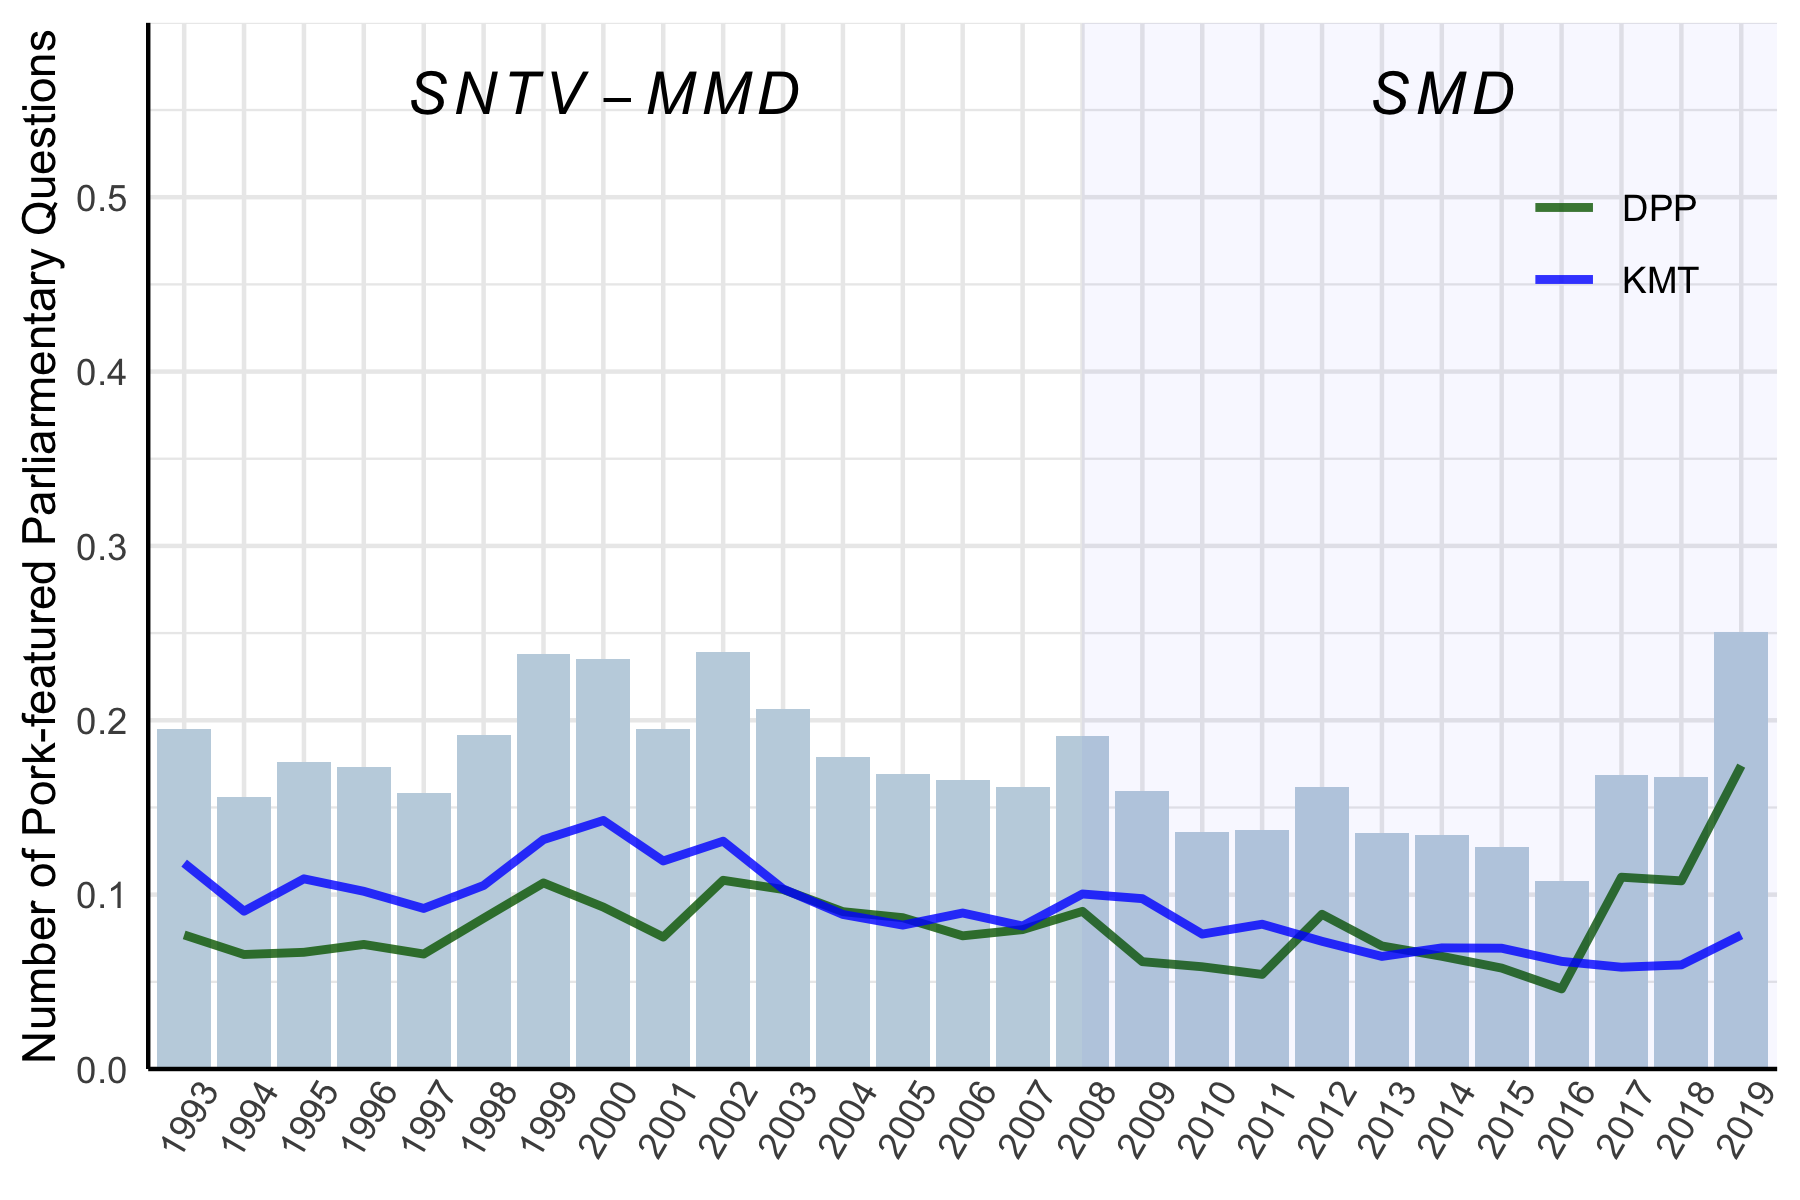
\includegraphics[width=7.2cm, height=6cm]{03-Chapter-Three/image/bigpqmean.png}
    \caption{Large Parties}
    \label{fig:meanporkbig}
    \end{subfigure}
    \centering
    \begin{subfigure}[t]{0.48\textwidth}
    \centering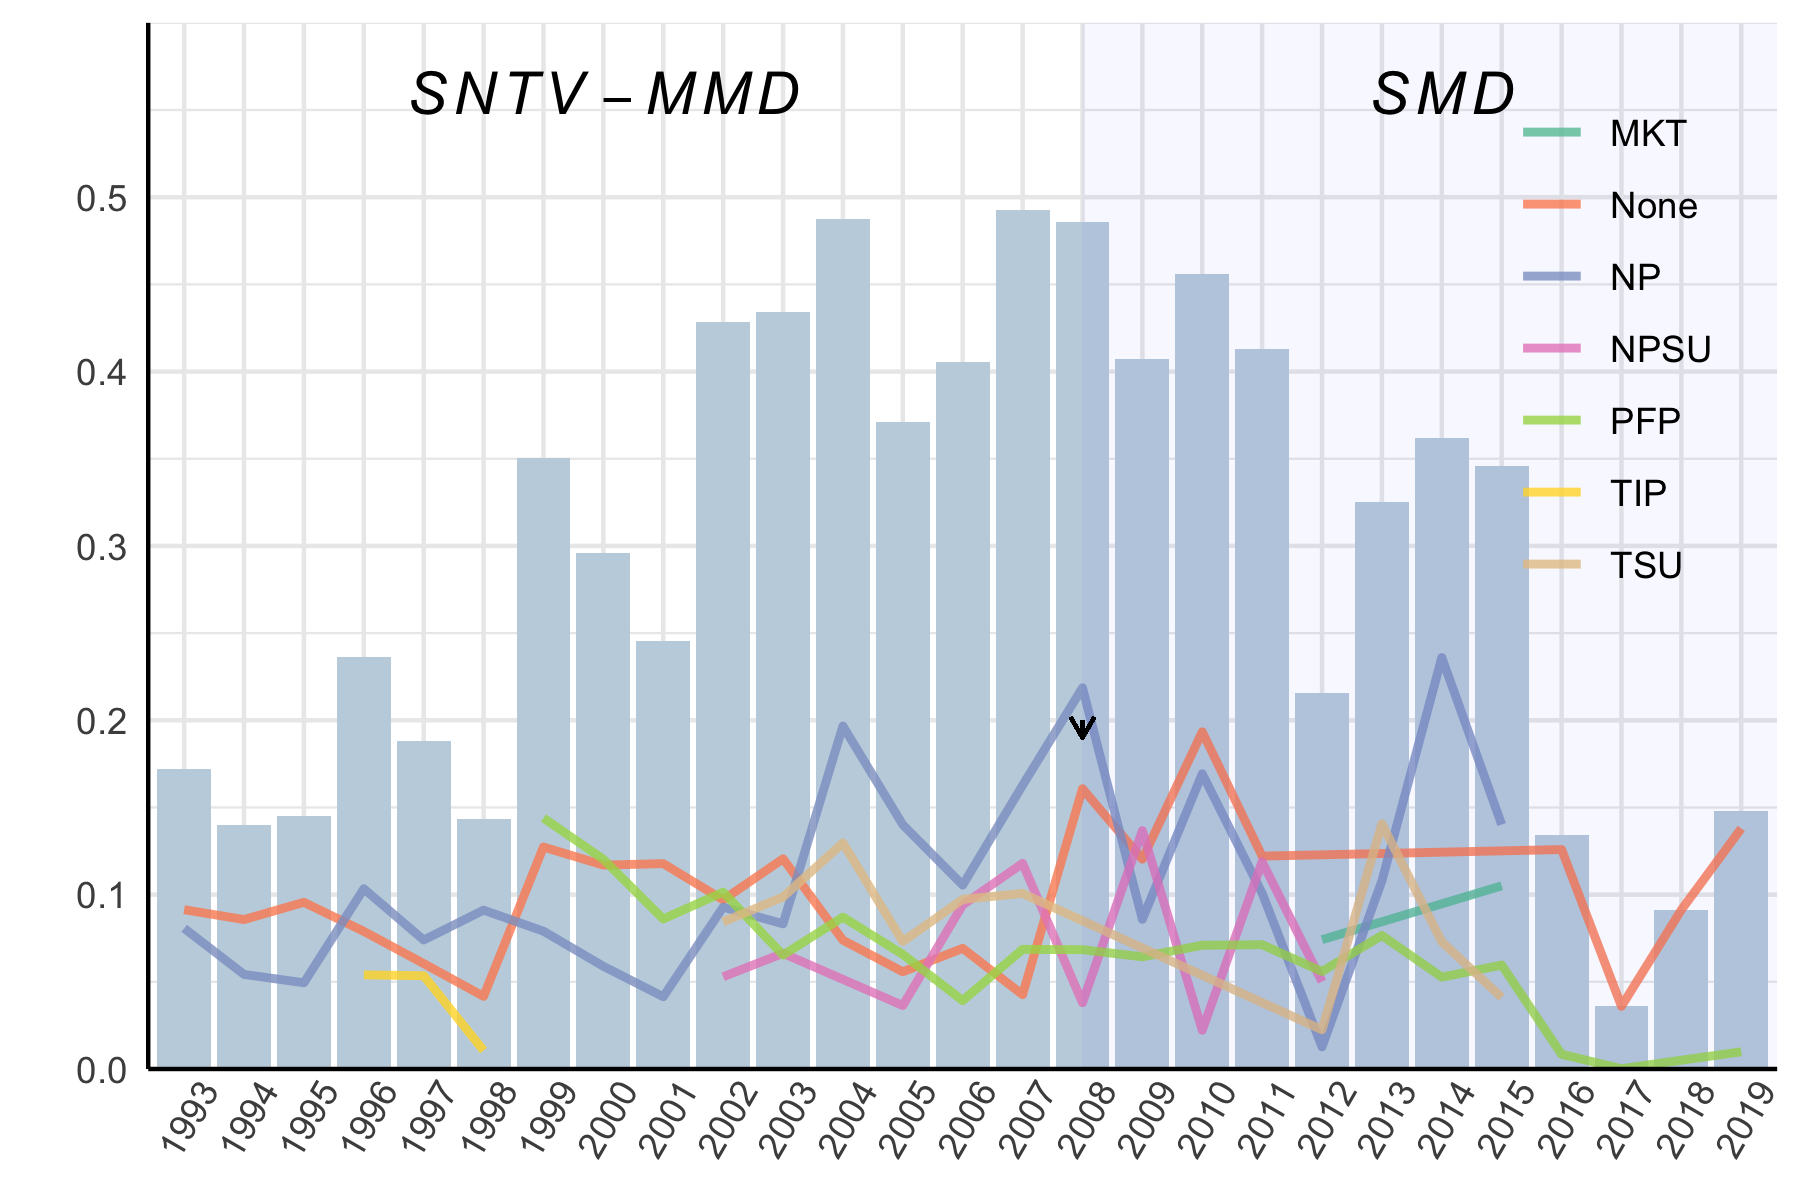
\includegraphics[width=7.2cm, height=6cm]{03-Chapter-Three/image/smallpqmean.png}
    \caption{Small Parties}
    \label{fig:meanporksmall}    
    \end{subfigure}
    \caption{The Mean Number of Pork Barrel Question by Years}
    \label{fig:meanpork}    
\end{figure}


\section*{\centering The Presence of the Electoral Reform}

How does the reform from SNTV-MMD to SMD-MMM change legislators' representation? To answer the question, I investigate to what extent the reform reduces legislators' incentive to ask pork-barrel questions. In total, legislators asked 116,248 questions throughout the reform transition from 1993 to 2020. While multiple plunges and surges between 2000 and 2015 reveal that the passage of years possibly affects the legislators' intention to propose the questions. To distinguish any irrelevant event to influence our analysis, I first calculated the mean of the pork features by an individual legislator at a quarterly unit and ran the following regression in \autoref{eqn:reg}, 

\begin{equation}
\begin{aligned}
 Pork_{i,t} = & \alpha_{0}+\alpha_{1}Electoral Reform_{t}+\alpha_{2t} +  \\
              & \alpha_{3}{(Electoral Reform_{t}\times{t})} +            \\
              & \theta C_{i,t}+ \epsilon_{it},
\label{eqn:reg}            
\end{aligned}
\end{equation}

where the dependent variable, $Pork_{i,t}$, is mean of pork-barrel questions aggregated at quarterly individual level, $ElectoralReformt_{t}$ is a dummy variable indicating whether the observation is  from the period of the post reform, $C_{i,t}$ includes fixed effects for municipality $i$ in election $t$, and $\epsilon_{it}$ is the error term. \autoref{tab:reg} shows a negative and significant effect on legislators' motivation to ask pork-barrel questions after reform, both for \textit{Full Model} and \textit{Large Parties}, suggesting that changing to SMD decreases legislators' incentives to pay attention to parochial interests. Thus, I find generally consistent empirical evidence in favour of \textbf{the Hypothesis \ref{h:h1}}. 

Yet, the heterogeneity issues resulting from natural disasters and political incidents occurred in years that could potentially influence legislators' incentive to ask specific questions or ask more (less) questions. For example, in 2006, a mass movement (\textit{Million Voices against Corruption, President Chen Must Go}) in Taipei Liberty Square led by former DPP Chairman Shih Ming-teh pressured President Chen Shui-bian to resign. This incident was in the media for more than a year, from 2007 to 2008, when the reform was just in practice. To diminish the problem concerning the heterogeneity, I control for the fixed effects from municipalities and legislators across the years. Still, the reform is statistically significant negative, and robust in models (2) and (4). 

As such, the empirical evidence shows that increases in time were associated with higher motivation levels to ask pork questions under the old system, SNTV-MMD, and lower levels under SMD. This suggests the institutional change reduces legislators' tendency to ask for the pork-barrel project between KMT and DPP, even if I introduce municipality dummies, legislator dummies, control for the passage of time and other demographics. 


\begin{sidewaystable}[!htbp]

% \begin{table}[h]
    \centering
    \caption{Regression Analysis for Pork-barrel Questions}
\scalebox{1}{
    \begin{threeparttable}
    \def\sym#1{\ifmmode^{#1}\else\(^{#1}\)\fi}
    \begin{tabular}{l*{6}{c}}
    \toprule 

                &\multicolumn{2}{c}{Full Observation} 
                &\multicolumn{2}{c}{Large Parties}
                &\multicolumn{2}{c}{Small Parties}\\
                 \cline{2-7}  \\
                &\multicolumn{1}{c}{Model  (1)}
                &\multicolumn{1}{c}{Model  (2)}
                &\multicolumn{1}{c}{Model  (3)}
                &\multicolumn{1}{c}{Model  (4)}
                &\multicolumn{1}{c}{Model  (5)}
                &\multicolumn{1}{c}{Model  (6)}\\                
                &\multicolumn{1}{c}{Interaction}
                &\multicolumn{1}{c}{+ Controls}
                &\multicolumn{1}{c}{Interaction}
                &\multicolumn{1}{c}{(+ Controls)}
                &\multicolumn{1}{c}{Interaction}
                &\multicolumn{1}{c}{(+ Controls)}\\
     \midrule


Reform          &  -14.052\sym{***}   &   -13.125\sym{***} 
                &  -14.959\sym{***}   &   -16.346\sym{***} 
                &  -11.180            &   4.954         \\
                &   (3.946)           &   ( 5.085)          
                &   (4.173)           &   ( 5.569) 
                &   (8.365)           &   (19.928)          \\


Year            &    -.006\sym{***}   &    -.006\sym{***}
                &    -.006\sym{***}   &    -.008\sym{***} 
                &    -.002            &    -.001             \\
                &     (0.001)         &    (0.001)     
                &     (0.001)         &    (0.001) 
                &     (0.002)         &    (0.003)            \\
                
Reform $\times$ Year   &    .006\sym{***}    &    .006\sym{***}
                &    .007\sym{***}    &    .008\sym{***} 
                &    .005             &   -.002                    \\
                &     (0.001)         &   (0.002)     
                &     (0.002)         &   (0.002) 
                &     (0.004)         &   (0.009)         \\

Constant        &   12.610\sym{***}   &    12.713\sym{***} 
                &   13.732\sym{***}   &    16.206\sym{***} 
                &    5.091            &     2.712          \\
                
                &   (2.129)           &   (2.735)          
                &   (2.408)           &   (3.672) 
                &   (5.614)           &   (6.546)          \\

     \midrule

District Fixed Effects&                     &   \checkmark         
                      &                     &   \checkmark   
                      &                     &   \checkmark      \\    
                     
Legislator Fixed Effects             &                     &   \checkmark         
                     &                     &   \checkmark   
                     &                     &   \checkmark      \\   
                     
The Reform Year      &    \checkmark      &   \checkmark         
                     &      \checkmark   &   \checkmark   
                     &    \checkmark         &   \checkmark      \\   
                     
Observations         &    4,252            &    4,252         
                     &    3,539            &    3,539
                     &    713              &    713        \\
Adjusted \(R^{2}\)   &    0.016         &    0.218
                     &    0.020         &    0.233   
                     &    0.003         &    0.179     \\
\bottomrule
\end{tabular}
     \begin{tablenotes}
     Note: * \(p<0.10\),** \(p<0.05\), *** \(p<0.01\). \\ Robust standard errors in parentheses. The district-level pork-barrel parliamentary question at quarter-yearly is regressed on year, electoral reform, and interaction between year and electoral reform, with and without fixed effect controls. The controls include fixed effects for electoral districts, municipalities, and individual legislators and the occurrence of the reform. 
     \end{tablenotes}
     \end{threeparttable}
     }\label{tab:reg}
% \end{table}
\end{sidewaystable}


To distinguish any possible effects from the passage of time and control for differences between municipality and legislators, I ran the same regression as above by using a subsample only including the large parties (KMT and DPP) and small parties. However, the presence of the reform has an insignificant impact on legislators from \textit{small parties}, revealing that the effects of institutional change do not substantively discourage most small-party members from asking pork questions. Under the SMD, the minority legislators were squeezed for living space in the legislature, which subsequently motivated them to make more efforts to appeal to parochial groups of voters and ask more pork-barrel questions to the government on behalf of their voters in the district. 

\section*{\centering Discussion}

This chapter contributes to the literature on electoral systems and political representation by demonstrating how the institutional change decrease legislators' incentive to run on their personal reputation by adopting electoral strategies that target the median voter. Combining a dedicated deep learning algorithm with robust regression analysis, I estimate the impacts of the electoral reform through SNTV-MMD to SMD on legislative behaviour. The results show that Taiwan's SMD diminishes legislators' motivation to mention pork-barrel features and increases their awareness of regulatory policies in written parliamentary questions. This finding is in line with a recent study by \citet{Catalinac2016, Ishima2020} showing that the single-member district system increases elected representatives' attention to national policies \citep{Catalinac2016}. Nevertheless, the institutional change has a moderate impact on legislators from smaller parties. This is due to the fact that the new system introduced in Taiwan is particularly disadvantageous to small parties \citep{Duverger1954, Reed2001, Huang2017, Bawn2003}, which deteriorates the effect of the reform on their political behaviours and electoral strategies with the constituencies. 

This chapter thus comes with some limitations. First, the fact that there has been a steady decrease in the total number of questions since 2003 despite the reform substantially impacting legislative representation is still noteworthy. In particular, social media in recent years has become an important platform for legislators to take positions and influence agenda setting \citep{Barbera2015, Barbera2019, Schurmann2022}. Additional limitations arise from the language transformation and its variation across times. As noted earlier in \autoref{sec:pqdata}, the pork barrel legislation from training data used in this chapter has been nearly ten years. The deep learning classifier learning patterns from the training set might fail to capture unknown concepts developed in the post-reform period. With BERT's self-attention mechanisms \citep{Vaswani2017}, the BERT-based framework may assist the machine classifier by simulating a similar skill set to human brains that can identify more complex or unseen concepts derived from the labelled data to understand the underlying pork barrel features.

Measuring legislators' preference towards constituencies under the different systems is essential to understanding the electoral system and the impacts on political representation. This chapter looks at an enduring myth about the impact of the 2008 electoral reforms in Taiwan. Although the reform, as scholars argue, some evidence indicates that SMD may not be as effective as initially presumed in solving drawbacks of the SNTV, such as factional politics and intraparty competition \citep[e.g.,][ ]{Wu2003, Batto2018}. The empirical evidence shows that increases in time were associated with lower motivation levels to run on personal reputation despite the fact that intense conflicts between parties when the reform occurred \citep{liao2020}. 